\documentclass[12pt,oneside]{book}
\usepackage{../thesis} % use thesis style file
\begin{document}

%===============================================================================
% TITLE PAGE / ABSTRACT / ACKNOWLEDGEMENTS / TABLE OF CONTENTS
%===============================================================================
\frontmatter % this is the stuff that comes before the real text:
%Here goes the title page:
\pagestyle{empty}
\begin{titlepage}
\begin{center}
\rule{5.75in}{1pt} \\
\vspace*{-0.125in}
{\large \doublespacing Wesleyan University} \hfill {\large \doublespacing The Honors College}
\rule[0.2in]{5.75in}{1pt} \\
\vspace*{0.8in}

% title
{\LARGE \singlespacing \bf 
  Using Vertical Structure to Infer \\
  the Dynamical Mass Hidden in \\
  the AU Mic Debris Disk
  } \\
\vspace*{0.05in}
\vspace*{0.10in}

{\large \vspace*{0.20in}  \singlespacing by \vspace*{.2in}
\\Cail Daley \\ Class of 2018\\}
\vspace*{0.25in}
\vspace*{0.8in}
{\large \singlespacing A thesis submitted to the\\ faculty of Wesleyan University\\ in partial fulfillment of the requirements for the \\ Degree of Bachelor of Arts\\ with Departmental Honors in Astronomy\\ \vspace*{-0.15in} }
\vspace*{.25in}
\rule{5.75in}{1pt} \\
\vspace*{-0.125in}
{\large \doublespacing Middletown, Connecticut \hfill April, 2018}
\rule[0.2in]{5.75in}{1pt} 
\end{center}
\end{titlepage}

\pagestyle{empty}
%\pagestyle{plain}

\mbox{}
\vspace{.75in}
\hrule

\vspace{2in}


%\begin{minipage}[c]{4in}
\begin{centering}
	\hspace{.25in} 
	\parbox{5in}{
		\noindent 
		\textit{We are just an advanced breed of monkeys on a minor planet of a very average star. But we can understand the Universe. That makes us something very special.}
		\vspace{3pt}

		\begin{flushright}
			{\sc {--Stephen Hawking}}\\
		%	{\textit{The Hitchhiker's Guide to the Galaxy}}
		\end{flushright}
	}
\end{centering}
\vspace{2.25in}
\hrule
\vfill



%\flushleft















\textwidth 5.750in \textheight=8.50in \headheight 0.0625in \topmargin 0.0in % book strict

% \chapter{Acknowledgements}

I would like to thank Meredith Hughes for being an amazing mentor through the process of teaching me to do advanced research, all the way from the crash course in radio astronomy at the beginning of my Junior year through this thesis. I'm blessed to have worked with such a dedicated advisor who cares so much about the learning process for each and every student. Going to Hawaii to observe at the SMA and Seattle for AAS were unforgettable experiences that not many undergraduates have, but those are really just cherries on top of the incredible sundae of knowledge, experience, and wisdom that you've passed on to me. 

Thanks to Seth Redfield for selling me on the astronomy program here at Wesleyan and getting me involved with the 24$''$ observing program. I may never live down getting flung from my chair as the monkey in an angular momentum demonstration he put me up to, but at least I'm better at ultimate frisbee. 

Thanks to Kevin Flaherty, for helping me out with everything from cluster computing to statistical tests, and to Roy Kilgard, for the endless patience in helping me with computer issues and always being fun to stop by and talk to. Thanks to Angelo Ricarte for writing the foundation of the modeling code that I used in this thesis. 

To Mom and Dad, thanks for giving me multiplication problems before bed to help me fall asleep, even if you didn't always know the correct answer. I wouldn't be who I am today without your love and guidance. Mira, you're the best sister a little bro could ask for. 

To the basement crew, thanks for endless entertainment in times of drastic procrastination, playing darts, and letting me fly the baby drone around the library when that was our workspace without going crazy (RIP baby drone. Both a sorry and a damn you to the Fisk Telescope for breaking the last propellor). 

\titlespacing*{\chapter}{0pt}{*2}{*3}

\tableofcontents \pagestyle{empty}

\mainmatter 
% headers
\pagestyle{fancy}
\fancyhf{}
\fancyhead[R]{\thepage}
\fancyhead[L]{\leftmark}
\renewcommand{\chaptermark}[1]{\markboth{\scshape \thechapter.\ #1} {}}

%===============================================================================
% SECTIONS
%===============================================================================

\chapter{Introduction}
\label{chapter: introduction}

\section{Origins and the Nebular Hypothesis}
\label{origins intro}

All peoples have origin stories to explain how their world came into being; within the confines of Europe, the cosmogonies of the Abrahamic religions and especially of Christianity supplied these origin stories for a long time.
The origin of the world lay in a seven-day period of creation during which God created everything out of nothing; the world was thought to have remained static since the moment of creation \citep{kragh17,luminet16}. 
The Solar System, too, was held to be a static, stable, and created system.
For example, physicist Issac Newton took the apparent regularity and even perfection of the planetary motions to be indicative of a divine origin.
German philosopher Immanuel Kant explains that, for Newton, the common motions of the planets could have only come about if there was mediating interplanetary material capable of generating a ``community of influence'' among the planets.
The absence of any such material suggested that ``the direct hand of God had arranged this order without the application of the forces of nature'' \citep[226-227]{kant_2012}.
However, Isaac Newton's own theory of mechanism, encapsulated in his three Laws of Motion, provided a new direction: force-interactions between bodies could change the state of a system over time.

Influenced by the spirit of Newtonian mechanism sweeping across Europe, a 31 year-old Kant proposed a ``nebular hypothesis'' in 1755.
Kant followed a line of reasoning running opposite to Newton's, taking the common motion of the planets and the lack of any mediating material to indicate that the Solar System must have been different in the past.
He imagined that all the matter currently locked up in planets, comets, and asteroids ``was dissolved into its elementary basic material at the beginning of all things,'' and was distributed across the current extent of the Solar System \citep[227]{kant_2012}.
In so doing Kant foreshadowed the modern concept of a ``minimum mass solar nebula,'' a cloud of gas and dust with at least enough material to produce the planets of our Solar System in their current configuration.
This dispersed, nebulous state envisioned by Kant was only temporary: ``In a space filled in such a way, universal rest lasts only a moment. The elements have essential forces to put each other into motion and they are a source of life for themselves. Matter immediately endeavours to form itself.''
Kant imagined that the Sun was born from local density enhancements in the protostellar nebula that attracted nearby particles, leading to ``the formation of a body in this centre point of attraction, which grows, so to speak, from an infinitely small seed in rapid steps'' \citep[][228-29]{kant_2012}.
``Great eddies of particles,'' would form around the Sun; particles with intersecting orbits would bump into each other and spiral inwards, leaving behind a flat disk of particles orbiting in circular, parallel orbits.
Local density enhancements would again cause these eddies to collapse upon themselves, forming planets that cleared the path of their orbits through gravitational attraction.

Kant's nebular hypothesis was independently conceived of by Pierre-Simon \\ Laplace, who laid out a more detailed model in his 1796 \textit{Exposition du Syst\`eme du Monde}.
Formulated more than one hundred years before Charles Darwin published \textit{On the Origin of Species}, the nebular hypothesis marks one of the first times an evolutionary worldview was introduced into the sciences.
In fact, Stephen Brush argues that the nebular hypothesis may have increased the acceptability of evolutionary frameworks such as Darwin's theory of biological evolution.
Astronomer F.R.~Moulton argues that the nebular hypothesis ``accustomed scientists to thinking of change in long periods of time and thus prepared the way psychologically for the theory of organic evolution'' \citep{brush87}.

Breaking with the Church-backed conception of a static universe, Kant argued for a radically different understanding of the creation and history of natural systems:
\begin{quote}
  \onehalfspacing
  Creation is not the work of one moment. 
  After it has made a beginning with the production of an infinity of substances and matter, it is effective throughout the entire sequence of eternity with ever increasing degrees of fruitfulness... 
  Creation is never complete. 
  It is true that it began once, but it will never stop. 
  It is always occupied with bringing forth more phenomena\footnote{Also ``emergences'' or ``entrances,'' in the sense of an actor making an entrance in a play.} of nature, new things and new worlds. \citep[][266-67]{kant_2012}
\end{quote}
I think Kant makes a very useful methodological point here: understanding something in nature cannot be reduced to the study of the period of its origin, whether it be seven days or millions of years.
Astrophysicist and cosmologist Fred Hoyle argues that ``[w]henever the word ‘origin’ is used, disbelieve everything you are told'' \citep{hoyle93}.
Rigorous interpretation of a natural system requires study of the phenomena that creation continues to ``bring forth'' even after the formation of the system, and of the often competing forces involved in the production of these phenomena themselves.

For example, understanding our Solar System---and the planetary systems around other stars---would not only require investigation of the first \SI{10}{Myr} during which the majority of planet formation occurs, but would take into account the many processes that continue to regulate such systems after the close of planet formation.
Interactions with the gaseous protoplanetary disk or with other planetary bodies can cause planets to ``migrate,'' moving closer or farther away from the host star; Neptune may have even switched places with Uranus at some point in the past \citep{lublow10,tsiganis05}.
Planet-disk interactions can also imprint gaps, spiral arms, and many other features onto disks \citep[see][]{hughes18}.
In this work, we aim to investigate the forces at work in the later stages of planetary system evolution, when planets are mostly formed but may still interact with their parent disks or experience heavy ``bombardment'' from scattered planetesimals \citep{wyatt2008}.

\section{Circumstellar Disks and the Collisional Cascade}
\label{disks, cascade intro}

Though Kant's model suffered from several faulty assumptions and lacked mathematical rigor, the nebular hypothesis remains the accepted theory dictating the formation and evolution of the Solar System.
In its current form, the nebular hypothesis could be outlined as follows; a visual representation is provided in Figure \ref{fig: evolution}.
An interstellar cloud or `nebula,' composed primarily of molecular hydrogen, becomes gravitationally unstable and begins to collapse upon itself.
Material accumulates at the center of the cloud, forming a dense protostellar core enveloped by infalling material.
Conservation of angular momentum causes the protostar's envelope to flatten into an accretion disk that deposits gas and dust onto the protostellar surface.
Eventually, the protostar becomes hot enough to fuse deuterium in its core and stellar winds clear away its envelope, leaving behind a `protoplanetary' or planet-forming disk \citep{shu87}.
Terrestrial planets grow from small dust grains through a series of low-velocity collisions between particles. 
When a planetesimal grows large enough to generate a significant gravitational field it experiences a period of runaway growth, followed by a period of oligarchic growth which ceases when the protoplanet clears its orbit of planetesimals \citep{chambers_exo}.
Simulations indicate that the runaway and oligarchic stages of planet formation last hundreds of thousands to millions of years after planetesimals are formed \citep{wetherill&stewart93,kokubo00}.
Gas giants form either by accreting additional gas from the circumstellar environment onto terrestrial cores, or by direct gravitational collapse from instabilities in the protoplanetary disk in a manner similar to that envisioned by Kant \citep{d'angelo10}.

Protoplanetary disks tend to be gas rich and optically thick.
As Kant predicted, matter falling onto the central star in a process known as accretion is in large part responsible for the dissipation of these disks; agglomeration of dust grains into planetesimals and eventually planets also depletes protoplanetary material and can open up gaps in the disk \citep{williams&cieza11}.
Photoevaporation, in which radiation from the star carries gas particles out of the system, is active throughout the lifetime of a protoplanetary disk and is thought to be responsible for quickly dissipating the disk once accretion halts \citep{ercolano&pascucci17,clarke01}.
These processes cause the primordial or first-generation material of the protoplanetary disk to dissipate, leaving behind only second-generation ``debris''---planets, asteroids, comets, dust, and sometimes gas \citep{hughes18}.
The resulting debris disks, optically thin and significantly less luminous than their protoplanetary counterparts, are found around at least 25\% of Solar-type stars and are likely to be as common as the exoplanetary systems with which they are thought to be associated \citep{montesinos16}.

  \begin{figure}
  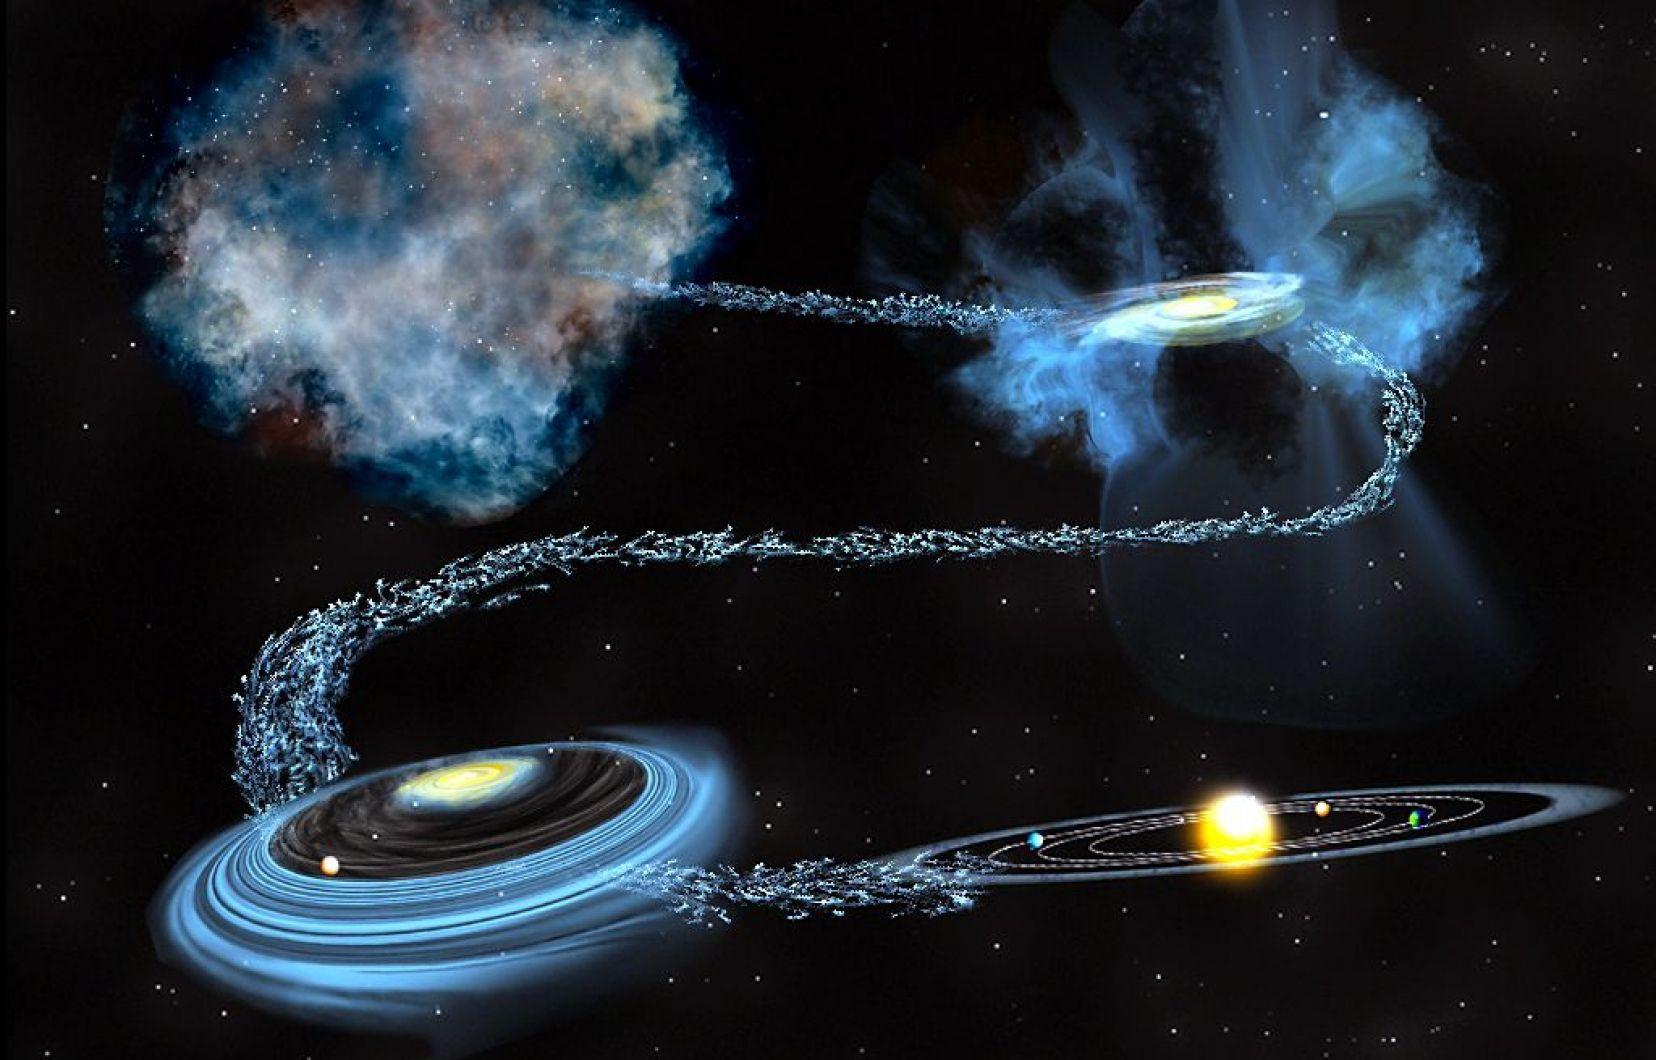
\includegraphics[width=\linewidth]{../figures/disk_evolution}
  \caption{Planetary system life sequence: (i) A nebula becomes gravitationally unstable and begins collapse. (ii) Angular momentum is conserved, and a flat accretion disk emerges from the infalling envelope. (iii) A protoplanetary disk forms around the pre-main-sequence star, and planetary bodies begin to form in the disk. (iv) The hot, dense protoplanetary material dissipates, leaving behind only planets and smaller planetesimals in a debris disk. Credit: Bill Saxton/NSF/AUI/NRAO}
  \label{fig: evolution}
\end{figure}

While planet formation and growth are thought to come to a close within \SI{400}{Myr} for terrestrial planets and within \SI{10}{Myr} for gas giants, circumstellar systems continue to evolve long after \citep{chambers13,d'angelo10}.
Debris disks can be found around stars as old as \SI{11}{Gyr}, although their incidence rate tends to decrease with age up to about \SI{1}{Gyr}. 
Debris disk dissipation seems to halt after this point \citep{sibthorpe18,matthews14}.
So what drives this dissipation?
Planetesimals in debris disks occasionally crash into each other, producing showers of dust in what is known as a ``collisional cascade'' \citep{wyatt2008}.
At the ``top'' of the cascade are planetesimals of size $a_{top}$, the largest bodies in the disk that can be collisionally disrupted.
Any bodies with size $a > a_{top}$ are too large to shatter if they collide with bodies inside the collisional cascade, and as such are ``above'' the cascade.
The collisional cascade grinds particles down until they reach the ``blowout size,'' where the force exerted by stellar radiation and winds exceeds the gravitational force exerted by the star.
Grains below the blowout size are quickly removed from the system, meaning that debris disks are perpetually eating away at themselves.
\cite{dohnanyi} was the first to mathematically characterize the steady-state collisional cascade and found that the differential size spectrum of bodies in the cascade can be described with a power law, $dN/da \propto a^{-q}$.
Integrating implies $N(a) \propto a^{1-q}$.
Here $N(a)$ is the number of bodies within a logarithmic size interval of $a$, or equivalently the number of bodies larger than $a$.
\cite{dohnanyi} found $q \approx 3.5$; more recent works have investigated generalizations of the canonical collisional cascade, for example allowing a size-dependent velocity distribution \citep{pan&schlichting12}.

Several processes regulate the velocities of planetesimals (and thus the destructive power of collisions) in a collisional cascade.
Larger planetesimals can gravitationally stir smaller bodies in their vicinity and so increase the velocity of planetesimals in the disk; on the other hand, dynamical friction can damp the velocities of larger bodies \citep{kenyon&bromley01}.
Dynamical friction is only effective for planetesimals with a non-negligible gravitational field, while collisional damping is effective for bodies of all sizes \citep{kenyon&luu99}.
All three effects play a role in determining the spatial distribution of dust in a debris disk undergoing a collisional cascade because they set the velocity dispersion of the disk's dust grains.
In particular, gravitational stirring isotropically scatters small dust grains both in the plane of the disk \textit{and} perpendicular to it.
The vertical height of a debris disk thus scales with the dynamical excitation of its constituent dust grains and the total mass of bodies gravitationally stirring the disk.
By studying the vertical structure of a debris disk, we can learn about the details of the collisional cascade that continually replenishes the disk's observable dust.

\section{Observing Debris Disks}
\label{observing intro}

\begin{figure}
  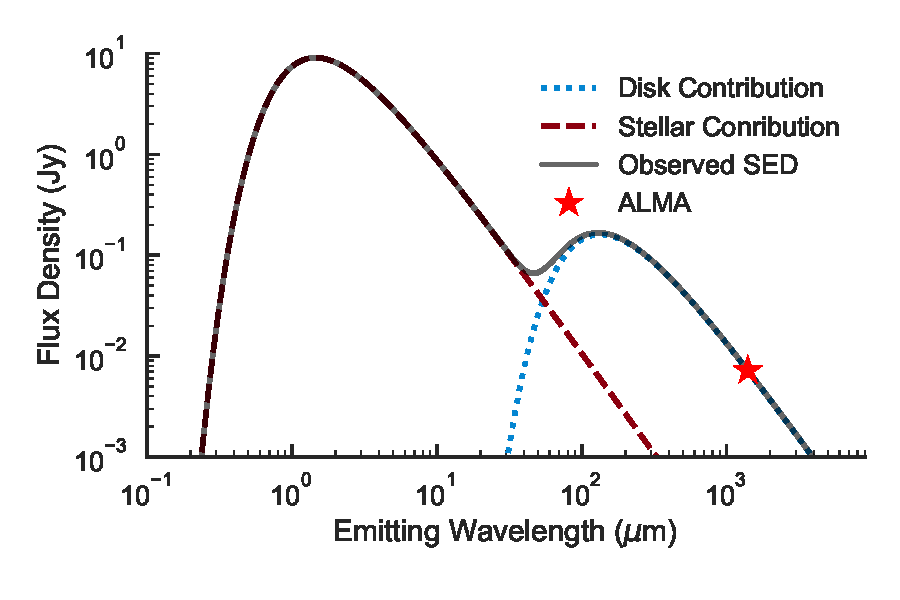
\includegraphics[width=\linewidth]{../figures/disk_SED}
  \caption{
  A toy model of a debris disk spectrum with parameters roughly matching those of AU Mic. 
  Stellar emission dominates at shorter (optical and near-infrared) wavelengths, while thermal imssion from the disk dominates beyond $\sim \SI{100}{\mu m}$.
  The red star marks the part of the spectrum seen by the ALMA observations discussed in \S \ref{chapter: observations}.
  }
  \label{fig: SED}
\end{figure}

The small dust grains produced by a collisional cascade can be observed at a wide range of wavelengths, and it is emission from such grains that allows us to detect debris disks around other stars.
At first glance this may seem counterintuitive, considering that for typical values of the collisional cascade size spectrum index $q$ the mass of dust particles is dwarfed by that locked up in larger planetesimals.
However the dust grains are responsible for the majority of the disk's surface density, and thus are the dominant source of emission.
The cool temperatures of debris disks---typically less than \SI{100}{K} for Solar-type stars---means that the dust particles emit blackbody radiation at far infrared and millimeter wavelengths.
Thermal emission from dust grains actually dwarfs stellar emission at longer wavelengths, creating a bump or `infrared excess' in the system's spectrum and spectral energy distribution (SED).
Debris disks have historically been detected in this manner; \cite{aumann84} was the first to do so.
Figure \ref{fig: SED} shows a toy model of a composite spectrum from a star-debris disk system, tuned to broadly match that of the AU Mic.

Spatially resolved observations can provide more detailed information across a wide range of wavelengths (Figure \ref{fig: observation comparison}).
At optical and near-infrared wavelengths dust grains are too cold to emit significant amounts thermal radiation, but they do scatter radiation from the central star; the spatial distribution of the smallest grains in the disk can thus be determined from short-wavelength scattered light images of the disk.
On the other hand, the development of high-sensitivity interferometric arrays such as the Atacama Large Millimeter/submillimeter array (ALMA) has significantly extended the range of wavelengths at which we can observe debris disks.
ALMA combines the signals from individual radio antennas (fifty-four \SI{12}{m} and twelve \SI{7}{m}) to detect millimeter sources with much greater sensitivity and resolution than would be possible with a single antenna.
Particles of dust are efficient emitters only if they are larger than the wavelength of the emitted light, so long-wavelength thermal emission seen by ALMA traces the larger dust grains that are more likely to be cospatial with the parent planetesimal population (e.g. Figure \ref{fig: observation comparison}d).

\begin{figure}
  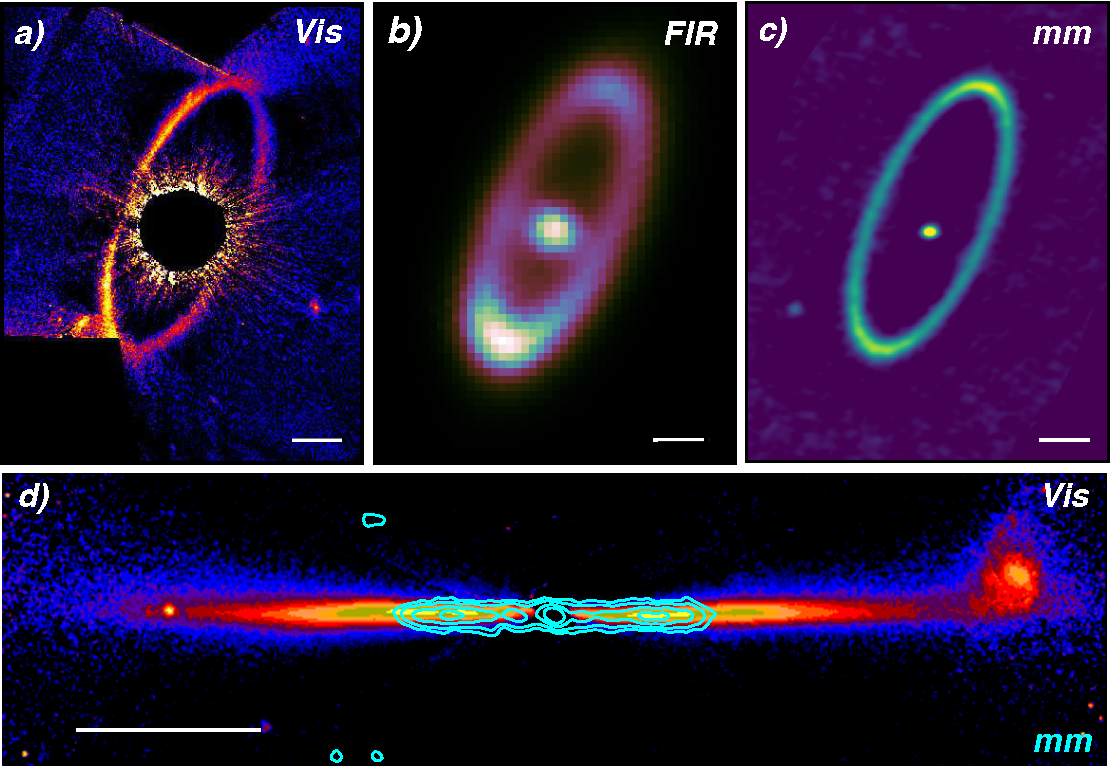
\includegraphics[width=\linewidth]{../figures/hughes_etal18_observation_comparison}
  \caption{
  An illustration of the effect of observing wavelength on apparent structure of debris disks, from \cite{hughes18}. 
  \textbf{Top:} the Fomalhaut debris disk.
  \textit{Hubble Space Telescope} (\textit{HST}) scattered light images trace small dust grains reflecting optical emission from the central star \citep[\textbf{a},][]{kalas13}, while longer-wavelength observations from \textit{Herschel} \citep[\textbf{b},][]{acke12} and ALMA \citep[\textbf{c},][]{macgregor17} detect the spatial distribution of thermally-emitting larger dust grains.
  \textbf{Bottom:} ALMA observations (contours, this work) trace larger grains orbiting within $\sim \SI{40}{au}$ of the star, while scattered light \textit{HST} images \citep[colormap,][]{schneider14} reveal a more extended population of small grains.
  }
  \label{fig: observation comparison}
\end{figure}

Our own Solar System boasts a debris disk with two distinct belts.
The innermost component can be seen from Earth as the faint glow of the zodiacal light, the only debris disk emission visible to the naked eye (Figure \ref{fig: zodiacal}). 
The zodiacal light is made up of starlight reflected off of countless dust grains in the inner solar system; most ($\sim 80\%$) of these grains are collisionally produced by Jupiter-family comets and subsequently scattered inwards by by Jupiter, but a small fraction ($\sim 10\%$) originate in the asteroid belt \citep{nesvorny10,wyatt2008}.
The second component of the Solar System, known as the Kuiper belt, extends from the orbit of Neptune (\SI{30}{au}) to slightly less than \SI{50}{au}.
The Kuiper belt is made up of planetesimals and collisionally produced dust that has been relatively unaffected by the planet formation that occurred in the inner regions of the Solar System.
Some Kuiper belt objects are quite large: for example Pluto, $\sim \SI{2400}{km}$ across, is a member of the Kuiper belt.
Debris disks around other stars often share the two-component structure of the Solar System's debris disk, but nearly all detected so far are at least an order of magnitude more luminous \citep{matthews14}.

\begin{figure}
  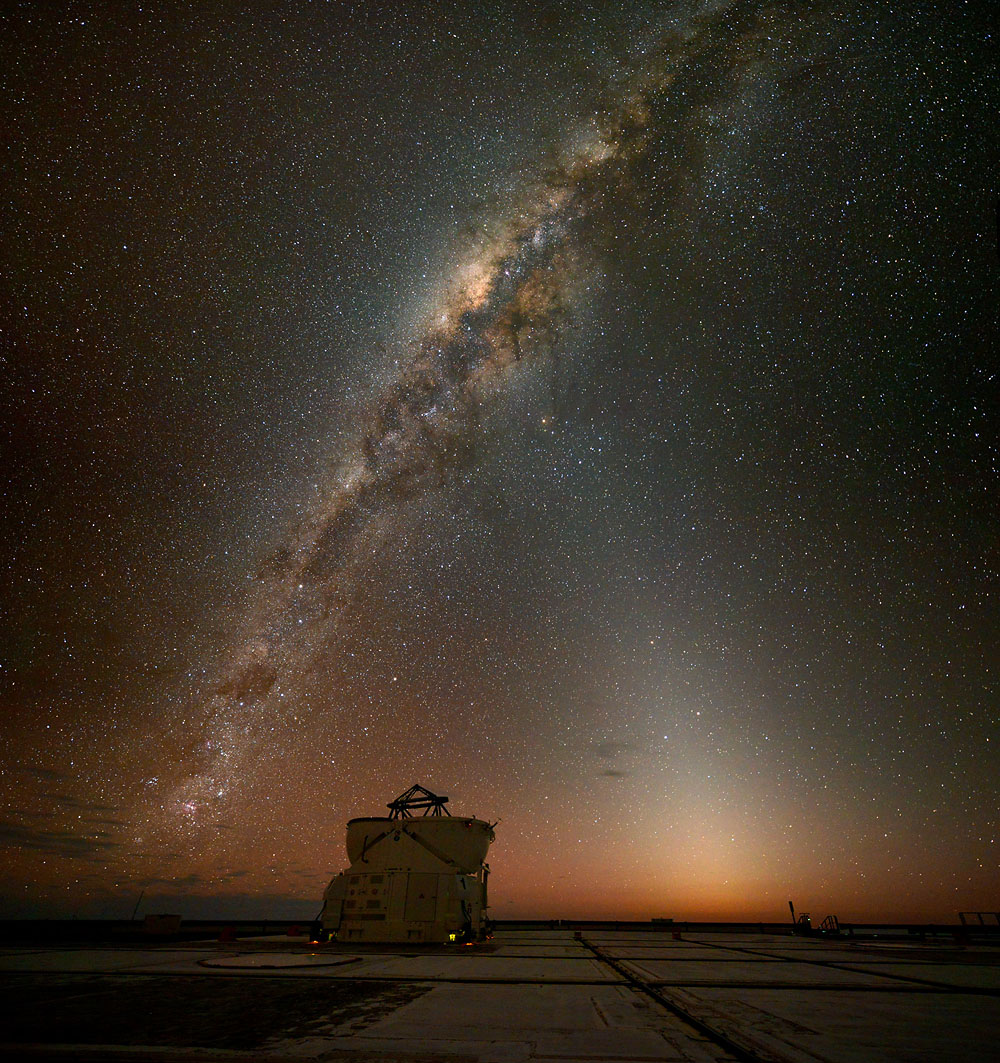
\includegraphics[width=\textwidth]{../figures/zodiacal_light}
  \caption{
  A view of the night sky over the Very Large Telescope in the Atacama Desert, Cerro Paranal, Chile. 
  The zodiacal light (also known as ``false dawn'') is visible as a slanted band of light extending up from the horizon towards the center of the Milky Way.
  Photo By Gerhard Hudepohl.}
  \label{fig: zodiacal}
\end{figure}

\section{The AU Mic Debris Disk}
\label{AU Mic intro}

Kuiper belt analogs, characterized by low optical depths and dust produced by destructive processes rather than agglomeration, can be found around many stars \citep{hughes18}.
A notable example is the edge-on debris disk around nearby (\SI{9.91}{pc}) M3IVe star AU Mic; its constituent dust particles are thought to be produced by a ``birth ring'' of parent planetesimals located at $\sim \SI{40}{au}$ \citep{vanleeuwen07, strubbe&chiang06}.
The first M star detected to have a far-infrared excess in its SED, AU Mic hosts one of the best-studied debris disks \citep[][; see Figure \ref{fig: SED}]{moshir90}. 
As a member of the $\beta$ Pic Moving Group, it is thought to be relatively young: $\SI{23 \pm 2}{Myr}$ \citep{binks&jeffries14,mamajek&bell14,malo14}. 
The disk around AU Mic was first resolved by \cite{kalas04} in scattered light, and a host of observations spanning the optical to the submillimeter have followed \citep{augereau&beust06,macgregor13,matthews15,schneider14,wang15}. 
Notably, the debris around AU Mic exhibits a so-far-unique time variability at scattered light wavelengths.
\cite{boccaletti15} identify five features---local intensity maxima offset from the disk midplane---on the SE side of the disk. 
These features are quickly moving away from the star along the disk midplane at projected velocities that are not consistent with Keplerian rotation; in fact, the outermost two features appear to be unbound from the star. 
Both dust emission from a localized source such as a planet \citep{boccaletti15,sezestre17} and collisional dust avalanches \citep{chiang&fung17} have been proposed to explain these features.

The proximity and edge-on inclination of the AU Mic debris disk allow its vertical structure to be resolved with relative ease.
As discussed in \S \ref{disks, cascade intro}, the vertical structure of a debris disk is related to the population of bodies stirring the collisional cascade; measuring the vertical thickness or ``scale height'' of AU Mic's debris disk thus provides a rare opportunity to learn about the mechanics of collisional cascades outside of the Solar System.
Such work has been undertaken by several authors using visible and infrared observations \citep{artymowicz97,thebault&augereau07,quillen07}.
However, \cite{thebault09} demonstrates that radiation pressure from the host star should excite the smallest dust grains, imparting a `natural' scale height to the disk even in the absence of large bodies dynamically stirring the disk. 
Thus longer-wavelength ($\lambda \geq \SI{50}{\mu m}$) observations are required to measure disk scale height as determined by dynamical stirring alone, since the grains dominating the emission at these wavelengths are large enough to be impervious to the effects of radiation pressure.

In this work we present new \SI{0.3}{\arcsecond} Atacama Large Millimeter/submillimeter Array \newline (ALMA) \SI{1.3}{mm} observations of the AU Mic debris disk. 
These observations represent a factor of $\sim 2$ improvement in both spatial resolution and rms noise relative to \cite{macgregor13}'s previous ALMA observations of the system, and our analysis indicates that the vertical structure of the disk is resolved with 4-6$\sigma$ confidence.
In \S \ref{chapter: observations} we present the new observations and describe the data reduction.  
\S \ref{chapter: results} quotes the basic observational results and compares the millimeter morphology of the disk with the morphology at shorter wavelengths.  
In \S \ref{chapter: analysis} we conduct a parametric exploration of a 2-dimensional disk model in order to investigate the degeneracy between vertical structure, radial structure, and viewing geometry.
In \S \ref{chapter: discussion} we discuss our results, particularly the constraints on the dynamical excitation of the disk imposed by our measurement of the scale height, and compare them to previous observations.
The results of our measurement of scale height and its implications for the total disk mass are summarized in \S 6.

\clearpage

\chapter{Observations}
\label{chapter: observations}
AU Mic was observed  with ALMA on three dates: 26 March 2014, 18 August 2014, and 24 June 2015 (see Table \ref{tab:observations}). 
The baseline lengths range between \SIlist{12;1320}{m}; the longest baseline among the three observations traces an angular scale of \SI{0.22}{\arcsecond} and a spatial scale of \SI{2.2}{au}.
All observations employed ALMA's 12m antennas and Band 7 receivers, including four independently tunable spectral windows. 
One spectral window was centered around the CO $J = (2-1)$ transition at a rest frequency of 230.538001 GHz, with a total bandwidth of 1.875 GHz and a channel spacing of \SI{0.6}{km/s}.
The remaining three spectral windows were configured to detect continuum emission with central frequencies of 228.5, 213.5, and 216.0 GHz, total bandwidths of 2 GHz, and channel spacings of \SI{21.7}{km/s}.

\begin{table}
  \centering
  \begin{tabular}{lrrrr}
  \toprule

  {Observational parameters}
                        & 26 March 2014 & 18 August 2014 & 24 June 2015 \\
  \cmidrule(lr){2-4}
  \cmidrule(lr){1-1}
  Antennas:             & 32           & 35            & 37             \\
  Baseline length (m):  & 12--406      & 19--1160      & 30--1320       \\
  On-source time (min): & 35           & 35            & 33             \\
  Flux calibrator:      & Titan        & J2056-472     & Titan          \\
  Bandpass calibrator:  & J1924-2914   & J2056-4714    & J1924-2914     \\
  Gain calibrator:      & J2101-2933   & J2101-2933    & J2056-3208     \\
  pwv range (mm):       &[0.63, 0.66]  & [1.58, 1.69]  & [0.67, 0.74]
  \vspace{1em}                                                          \\

  {Imaging parameters} &&&                                              \\
  \cmidrule(lr){1-1}
  Beam size (arcsec): & 
    $1.27\times0.74$ & 
    $0.33\times0.30$ & 
    $0.47\times0.31$                                                    \\
  Peak intensity (\si{\mu Jy / beam}): & 630 & 240 & 320                \\
  rms noise (\si{\mu Jy / beam}):      &  30 &  30 &  20                \\
  \bottomrule
  \end{tabular}

	\caption{
  Observational and imaging parameters for the three datasets used in this work. 
  Images were created using the \texttt{CASA} task \texttt{tclean} with natural weighting.}
  \label{tab:observations}
\end{table}

Calibration, reduction, and imaging were carried out using the \texttt{CASA} \citep{mcmullin07} and \texttt{MIRIAD} \citep{sault95} software packages. 
Standard ALMA reduction scripts were applied to the datasets: phase fluctuations/decorrelations introduced by the atmosphere and electronics were corrected via gain calibration and water vapor radiometry tables, while system temperature calibrations were performed to account for variations in atmospheric and instrument conditions. 
Flux calibrations allowed the raw data to be accurately converted into flux densities, and bandpass calibrations were applied to account for frequency dependence in the amplitudes and phases caused by the atmospheric transmission spectrum and instrumental effects.
The flux calibration is subject to a 10\% systematic uncertainty.
In addition to these standard procedures, the weights of the visibilities were recalculated using the variance around each baseline as in \cite{flaherty17}.

During the last segment of the June observation (04:23:38-04:29:58 UT), the host star flared. 
To determine the flux of the flare as a function of time, we binned the data into one-minute intervals using the \texttt{CASA} task \texttt{split} and fit a point source in each bin to baselines between \SI{100}{\kilo \lambda} and \SI{1400}{\kilo \lambda} with \texttt{uvmodelfit}. 
Because the Fourier transform of a point source is constant across all spatial frequencies, the chosen baseline range excludes the shortest spatial frequencies ($< \SI{100}{\kilo \lambda}$) that trace extended structure while 
allowing the compact stellar emission traced by the longer baselines to be fit directly in the visibility domain.
The resulting flare fits can be found in Table \ref{tab:flare fluxes}. 
We exclude from our analysis the seven minutes during which the flare occurred, as it proved difficult to separate the stellar emission from the disk emission while it was changing so rapidly.

\begin{table}	
  \centering
  \begin{tabular}{lr}
    \toprule
    Time (UTC) & Point-source Flux ($\mu$Jy) \\
    \midrule
    03:45:0--04:20:0 (no flare) & ($4.1 \pm 0.2)  \times 10^2$\\
  	4:23:38--4:24:00 & $(9.2 \pm 1.7) \times 10^2$ \\
  	4:24:00--4:25:00 & $(1.146 \pm 0.010) \times 10^4$ \\
  	4:25:00--4:26:00 & $(3.59 \pm 0.10) \times 10^3$ \\
  	4:26:00--4:27:00 & $(1.58 \pm 0.10) \times 10^3$ \\
  	4:27:00--4:28:00 & $(4.50 \pm 1.0) \times 10^2$ \\
  	4:28:00--4:29:00 & $(4.60 \pm 1.0) \times 10^2$ \\
  	4:29:00--4:29:58 & $(5.20 \pm 1.0) \times 10^2$\\
    \bottomrule
  \end{tabular}
	\caption{Central point source flux before and during the June flare}
  \label{tab:flare fluxes}
\end{table}


Since AU Mic is a high proper motion system, its equatorial coordinates changed significantly over the 1.5 years between first and last observations.  
We were able to obtain a more precise alignment of the datasets from the bright chromospheric emission of the central star than from the measured proper motion.
We fit an image-domain elliptical Gaussian to a small region around the star on each date with the task \texttt{imfit}, and used the centroid of the Gaussian fit to define the star position.
Each dataset was then phase-shifted using the task \texttt{fixvis} so that the pointing center of the data was the same as the fitted star position.
We note that the exclusion of the flare changed the centroid of the Gaussian fit for the June observations by \SI{0.71 \pm 0.018}{au} (18\% of the synthesized beam) although the errors reported here, derived from the \texttt{imfit} uncertainties, are a factor of five smaller than those given by the ratio of beam size to SNR.
This change in the fit stellar location could be explained if the flare were not symmetric with respect to the star.

Imaging was performed using standard Fourier inversion methods as implemented in the \texttt{CASA} task \texttt{tclean}. 
Two weighting schemes were used: (i) natural weighting with no taper to trace the small-scale disk structure and (ii) natural weighting with a \SI{200}{k\lambda} Gaussian taper applied to long baselines to bring out the disk emission on larger spatial scales. 
In scheme (i) the rms noise $\sigma$ was \SI{15}{\mu Jy / beam} and the restoring beam was $\SI{0.52}{\arcsecond} \times \SI{0.39}{\arcsecond}$ with a position angle (PA) of \ang[angle-symbol-over-decimal]{77.9}. 
In scheme (ii), the corresponding values are \SI{20}{\mu Jy / beam}, $\SI{0.87}{\arcsecond} \times \SI{0.71}{\arcsecond}$, and \ang[angle-symbol-over-decimal]{80.8}
Because the \texttt{CASA} task \texttt{tclean} preserves pointing center offsets when converting several visibility datasets into an image, it was necessary to combine the data into a single file (with a common pointing center) before cleaning in order to account for the offset in phase center between datasets. 
This was done using the task \texttt{concat}, which combines datasets with pointing centers aligned so long as their pointing centers do not differ by a value greater than the parameter \texttt{dirtol}.

\clearpage
\chapter{Results}
\label{chapter: results}

\begin{figure}
  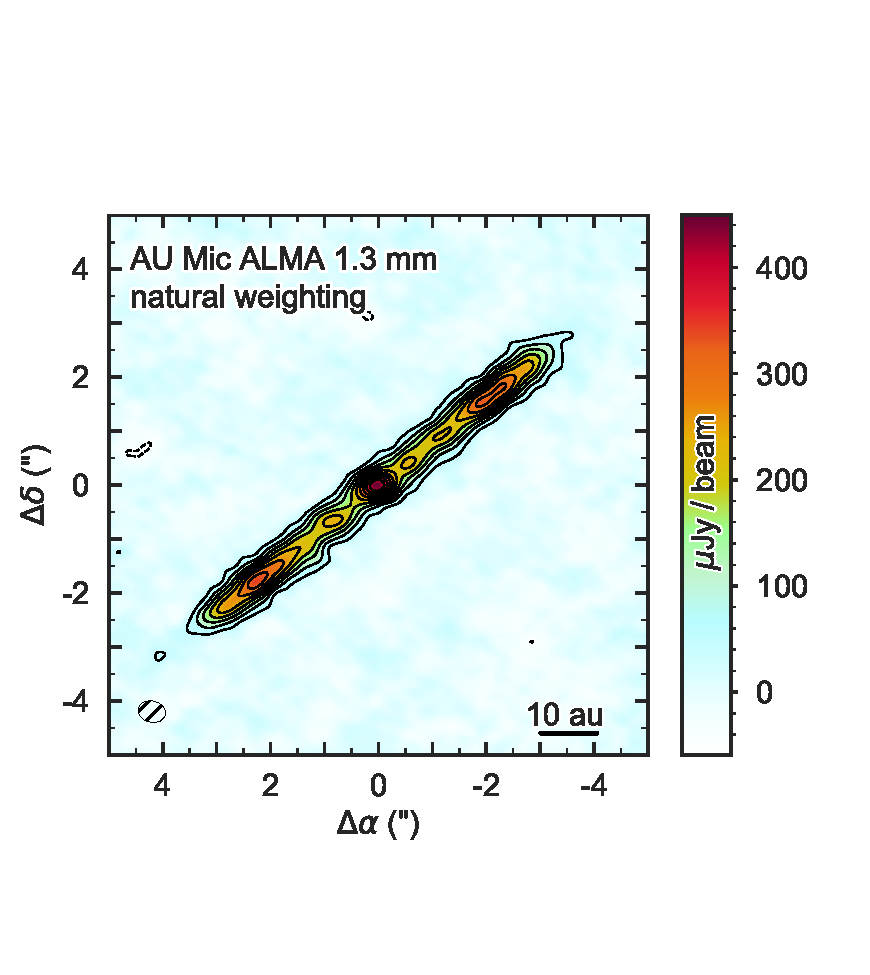
\includegraphics[width=\linewidth]{../figures/aumic_imaged}
  \caption{The AU Mic system imaged by ALMA at a wavelength of \SI{1.3}{mm}, using natural weighting with and without a Gaussian taper on the long baselines. 
  For the untapered weighting, the rms noise is \SI{15}{\mu Jy / beam} and the restoring beam has dimensions $\SI{0.52}{\arcsecond} \times \SI{0.39}{\arcsecond}$ with a PA of \ang[angle-symbol-over-decimal]{77.9}.
  The corresponding values for the tapered weighting are \SI{20}{\mu Jy / beam}, $\SI{0.87}{\arcsecond} \times \SI{0.71}{\arcsecond}$, and \ang[angle-symbol-over-decimal]{80.8}. 
  Contours are integer multiples of the three times the rms noise.
  The hatched ellipse in the bottom left of each pane designates the size and shape of the restoring beam.
  }
  \label{fig: aumic_imaged}
\end{figure}

Figure \ref{fig: aumic_imaged} shows the combined dust continuum emission from all three observations at \SI{1.3}{mm}; chromospheric emission from the M star is visible as a point source at the center of the image \citep{cranmer13}. 
The peak signal-to-noise ratio of dust emission is $\sim 23$.
Using the \texttt{MIRIAD} task \texttt{cgcurs}, we measure an integrated flux of \SI{4.97 \pm 0.08}{\milli Jy} enclosed within the $3\sigma$ contours of the naturally weighted image.  
Note that this value represents the combined emission from the disk \textit{and} the star. 
Faithfully disentangling the two components proved difficult, both because stellar and disk emission are blurred together in the central beam and because the stellar flux varied significantly across the three nights of observation (Table \ref{tab: params}).
Consequently, the most accurate way to isolate the disk flux from the stellar contribution is through parametric modeling (see \S \ref{chapter: analysis}) where the two components can be specified separately; our modeling yields a disk flux of \SI{4.8 \pm 0.2}{mJy}.
The ansa to the NW exhibits a maximum flux density of \SI{330 \pm 15}{\mu Jy/beam} at a separation of \SI{24.8 \pm 0.2}{au} and PA of $\ang[angle-symbol-over-decimal]{128.2} \pm 0.4$, while the ansa to the SE exhibits a maximum flux density of \SI{340 \pm 15}{\mu Jy} at a separation of \SI{29.0 \pm 0.2}{au} and PA of $\ang[angle-symbol-over-decimal]{128.7} \pm 0.4$. 
The peak flux densities of the ansae differ by less than the rms noise, indicating that there is no significant difference in brightness between the two limbs of the disk.
Indeed, the apparent flux asymmetry in these data is in the opposite direction of the apparent flux asymmetry in \cite{macgregor13}, providing further circumstantial evidence that there is no significant flux asymmetry at millimeter wavelengths. 
Additionally, the discrepancy in position angle between the two peaks falls within the estimated uncertainties and so we are not able to confirm the scattered light PA offset observed by \cite{boccaletti15}. 

\begin{figure}
  \centering
  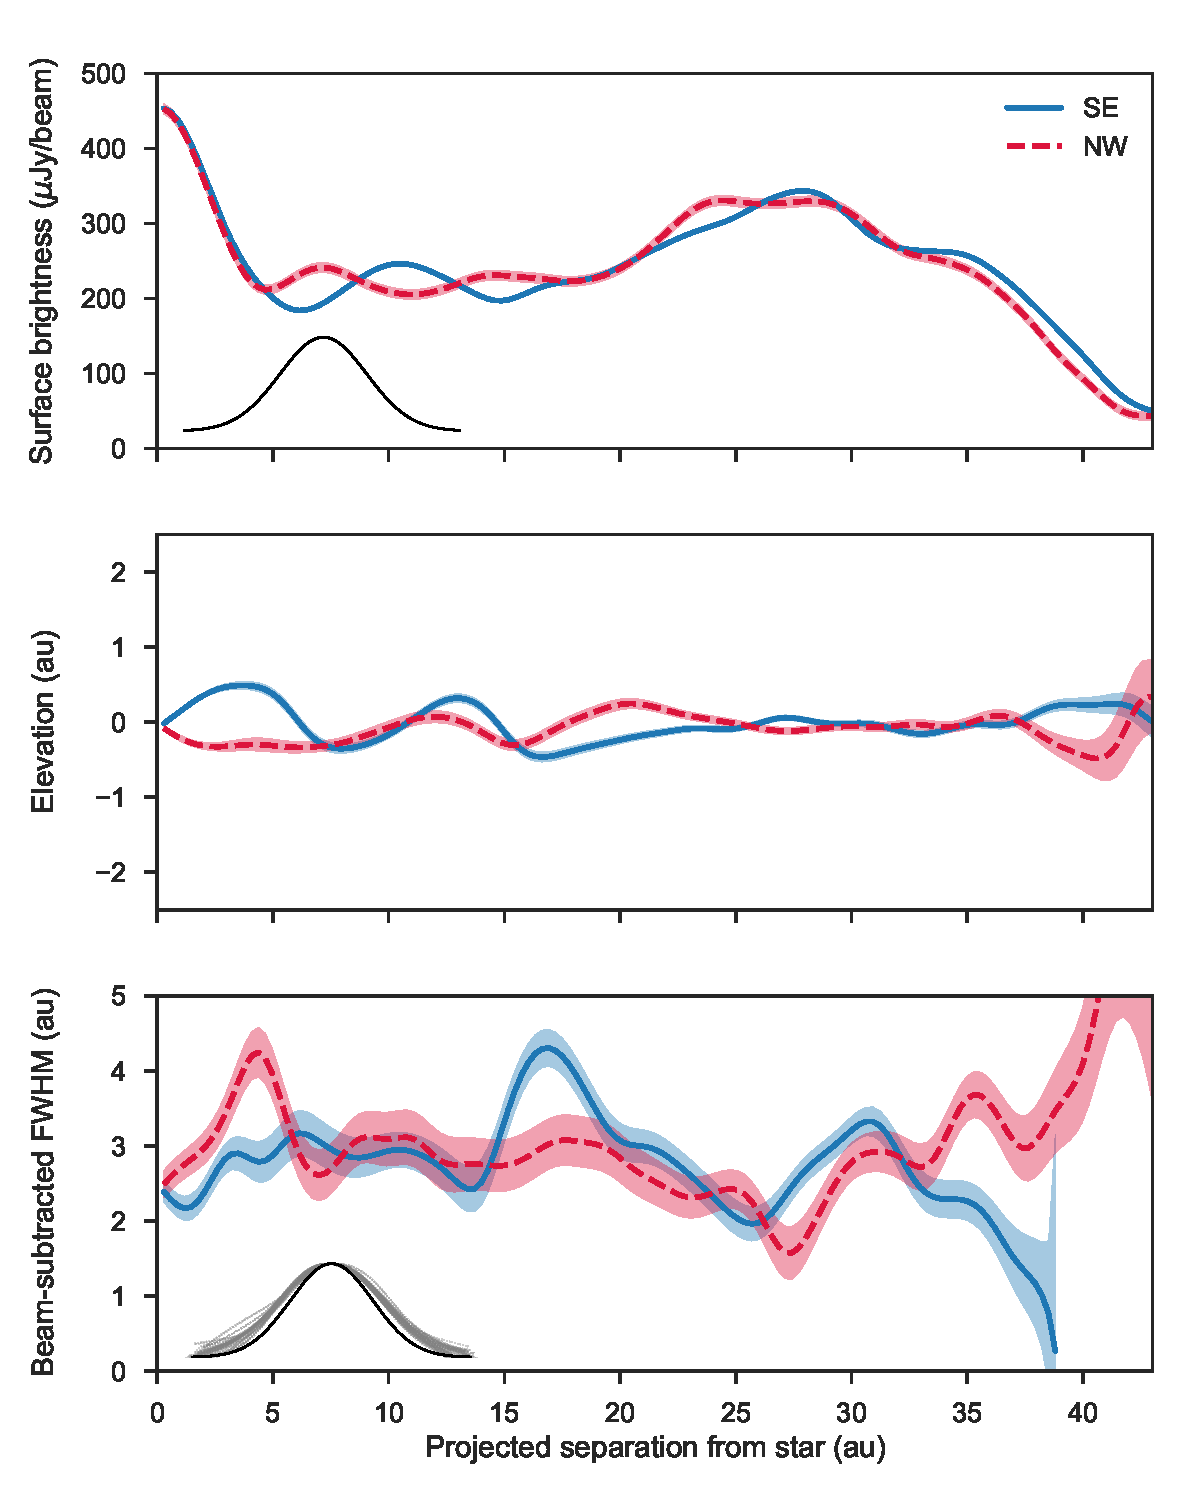
\includegraphics[width=.75\linewidth]{../figures/boccaletti_plots}
  \caption{
  Image-domain analysis of the AU Mic debris disk radial and vertical structure. 
  The solid blue line shows the southeast limb of the disk, while the dashed red line shows the northeast limb.
  From top to bottom, the three panes show i) the disk spine surface brightness with errors given by the rms noise, ii) the disk spine deviation from the midplane, and iii) the disk FWHM as a function of projected separation from the star. 
  The Gaussian traced by the dotted line in the first pane shows the projected width in the radial direction of the naturally weighted synthesized beam of the combined dataset.
  The fact that the image-domain vertical height of the disk is in excess of the beam contribution implies that our data spatially resolve the vertical structure of the disk.} 
  \label{fig: boccaletti}
\end{figure}

The vertical and radial structure of AU Mic's disk is traced in Figure \ref{fig: boccaletti}. 
At each radial location along the disk major axis, a one-dimensional Gaussian was fit to the vertical surface brightness profile.
The top, center, and bottom panes correspond respectively to the amplitude, centroid, and beam-subtracted FWHM of the Gaussian fits. 
Broadening effects of the synthesized beam in the vertical direction have been removed by subtracting in quadrature the Gaussian beam FWHM from the Gaussian fit FWHM.
In more physical terms, the three panes represent the intensity at the location of the disk ``spine,'' the spine's elevation from the midplane, and the disk FWHM.
We were unable to detect (in either the combined dataset or the three individual epochs) the intensity variations or excursions of the disk spine from the midplane that characterize the fast-moving features observed by \cite{boccaletti15}.
This is not entirely surprising, as both \cite{sezestre17} and \cite{chiang&fung17} suggest that the clouds are composed of sub-micron-sized grains which do not emit efficiently in the millimeter.

The disk is resolved across $\sim 17$ beams along the major axis, and cursory image-domain analysis indicates the disk is marginally resolved perpendicular to the major axis as well (Figure \ref{fig: boccaletti}, bottom pane).
$3\sigma$ emission as determined from the surface brightness profile in Figure \ref{fig: boccaletti} extends to a radial distance of $\sim \SI{43}{au}$ on the NW side and $\sim \SI{46}{au}$ on the SE side. 
We note the presence of local intensity maxima, nearly symmetric about the star at a distance of $\sim \SI{10}{au}$; it is unclear if these are real features of the disk or are artifacts of the rms noise or cleaning process. 
We examine the significance of these features in \S \ref{chapter: analysis}.


\clearpage
\chapter{Analysis}
\label{chapter: analysis}
Previous studies of the scale height of debris disks have demonstrated a degeneracy between vertical structure, radial structure, and viewing geometry \citep[e.g.,][]{milli14}.  
In light of this, we adopt a modeling approach that combines appropriate ray tracing methods with a Markov Chain Monte Carlo (MCMC) algorithm in order to investigate the degree to which these known degeneracies impact our ability to measure the vertical structure of the disk.  

\section{Modeling Formalism}

We use the parametric structure and ray tracing disk code described in \cite{flaherty15}, itself an adaptation of earlier work by \cite{rosenfeld13}.
Synthetic sky-projected images are generated from an assumed temperature and density structure and are subsequently Fourier transformed to create model visibilities that can be directly compared to the interferometric data.

We assume the disk to be azimuthally symmetric and vertically isothermal. 
The disk vertical structure is set by the aspect ratio $h = H(r)/r$. 
At a given radius $r$, the vertical density profile is assumed to be Gaussian with a standard deviation equal to the scale height $H(r)$.
The dust opacity is set to \SI{2.3}{\cm^2.\gram^{-1}} \citep{beckwith90}, placing the model disk in the optically thin regime for the range of dust masses explored.
For an optically thin disk, the observed thermal emission is determined by both the surface density and temperature of the dust; to break the degeneracy between these two parameters, we assume that the dust grains are in blackbody equilibrium with the central star.
Thus the dust temperature at a distance $r$ from the host star is given by
\begin{align}
  T_{dust} (r) &= \left( \frac{L_{\star}}{16 \pi r^2 \sigma} \right)^{1/4}
\end{align}
where $L_{\star}$ is the bolometric luminosity of the star and $\sigma$ is the Stefan-Boltzmann constant. We assume that the radial surface density takes the form of a power law: 
\begin{align}
  \Sigma(r) &= 
  \begin{cases}
    \Sigma_c \, r^{p} \; \; \; \; & r_{in} \leq r \leq r_{out} \\
    0 \; \; \; \; &\mbox{otherwise} 
  \end{cases}
\end{align}
where $p$ is the power law exponent, and $r_{in}$ and $r_{out}$ are the disk inner and outer radius. 
$\Sigma_c$ normalizes the surface density structure for a given total dust mass $M_{dust}$:
\begin{align}
\Sigma_c &= \frac{M_{dust} \left(p + 2 \right)}{2 \pi \left[ r_{out}^{(p+2)} - r_{in}^{(p+2)} \right]}.
\end{align}

The observed disk PA and inclination $i$ are free parameters.
We adopt a stellar luminosity of \SI{0.09}{L_\sun} \citep{plavchan09} and a distance to the star of \SI{9.91 \pm 0.10}{pc} \citep{vanleeuwen07}; the observed \SI{1.3}{mm} stellar flux $F_\star$ is left as a free parameter for each observation date.
We note that the uncertainty in the stellar distance could affect the modeled disk mass and disk radial extent, while the 10\% systematic flux uncertainty could affect the modeled disk mass and stellar flux.
The spatial resolution of the resulting model sky image is set to \SI{0.3}{au} per pixel, chosen to be $\sim \SI{10}{\percent}$ of the spatial scale sampled by the longest baseline in the data. 
After the model image is generated by the ray tracing code, it is Fourier transformed into the visibility domain and sampled at the same spatial frequencies as the ALMA data with the \texttt{MIRIAD} task \texttt{uvmodel}.
This allows the model to be compared directly to the interferometric data, for which the uncertainties are better characterized.
A $\chi^2$ metric is used to asses the quality of the fit.

We explore the parameter space of the model using the affine-invariant formulation of the MCMC algorithm described by \cite{goodmanweare10} and implemented in Python as \texttt{emcee} \citep{foreman-mackey13}.  
MCMC routines sample parameter space such that the density of samples in a given region is proportional to the local probability density, allowing estimation of the posterior probability functions themselves.
The process therefore not only identifies regions of high probability in parameter space, but also allows uncertainties and degeneracies between parameters to be determined from the correlations between the posteriors of each parameter. 
We assume uniform priors for all parameters; the dust mass was sampled in logarithmic space, formally equivalent to assuming a log uniform prior.
No prior bounds were placed on the logarithm of the dust mass.
Priors placed on the stellar flux and disk inner radius, width, and aspect ratio ensured that these parameters were always greater than zero, while the prior placed on the power law exponent ensured $-5 < p < 10$.
The inclination was confined to the range $\ang{0} < i < \ang{90}$, and the position angle to $\ang{1} < \text{PA} < \ang{360}$.
We performed several MCMC runs in order to investigate a variety of model formalisms. 
All runs used 50 walkers, and $10^5$ samples were drawn from each run to allow accurate statistical comparison between runs.


\begin{figure}
  \centering
  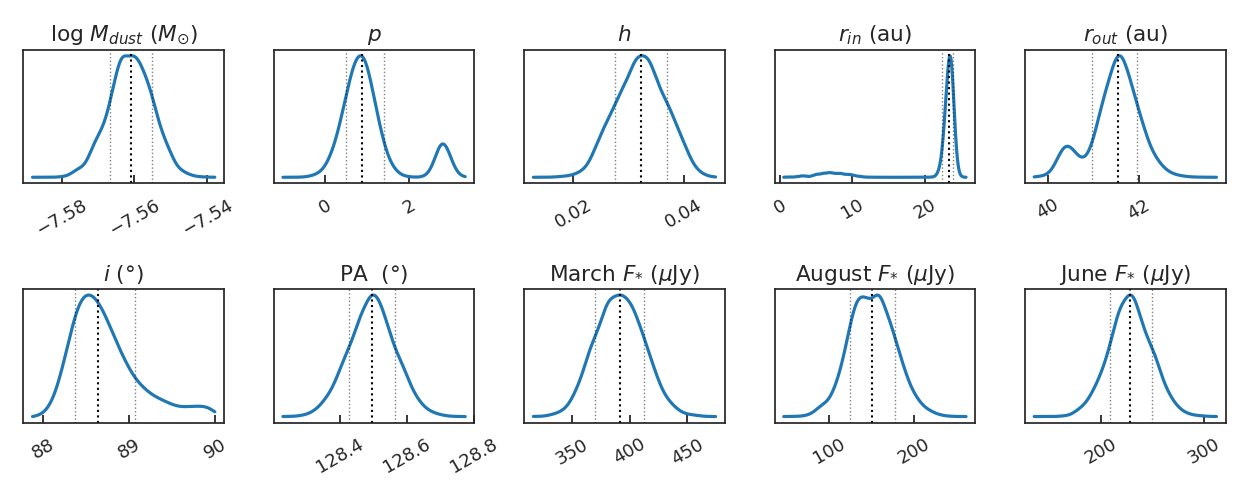
\includegraphics[width=\linewidth]{../figures/fiducial_kde}
  \caption{Kernel density estimates of the marginalized posterior probability distributions for the fiducial run. The central dashed line designates the median of each distribution while the outer lines mark the 16th and 84th percentiles ($1\sigma$ confidence intervals).}
  \label{fig: kde}
\end{figure}

Initially we varied ten parameters: the logarithm of the disk dust mass \linebreak ($\log M_{dust}$), the disk inner radius ($r_{in}$), width ($\Delta r$), power law exponent ($p$), scale height aspect ratio ($h$), inclination ($i$), position angle (PA), and finally a separate stellar flux ($F_\star$) for each of the three observation dates. 
After the fact, the posterior distribution for $\Delta r$ was replaced by the outer radius posterior $r_{out} = r_{in} + \Delta r$ to allow for easier interpretation.
This model formalism resulted in a best-fit $\chi^2$ value of 626163.598 (reduced $\chi^2=2.053$), and we treat this parameterization as our fiducial model.

\begin{figure}
  \centering
  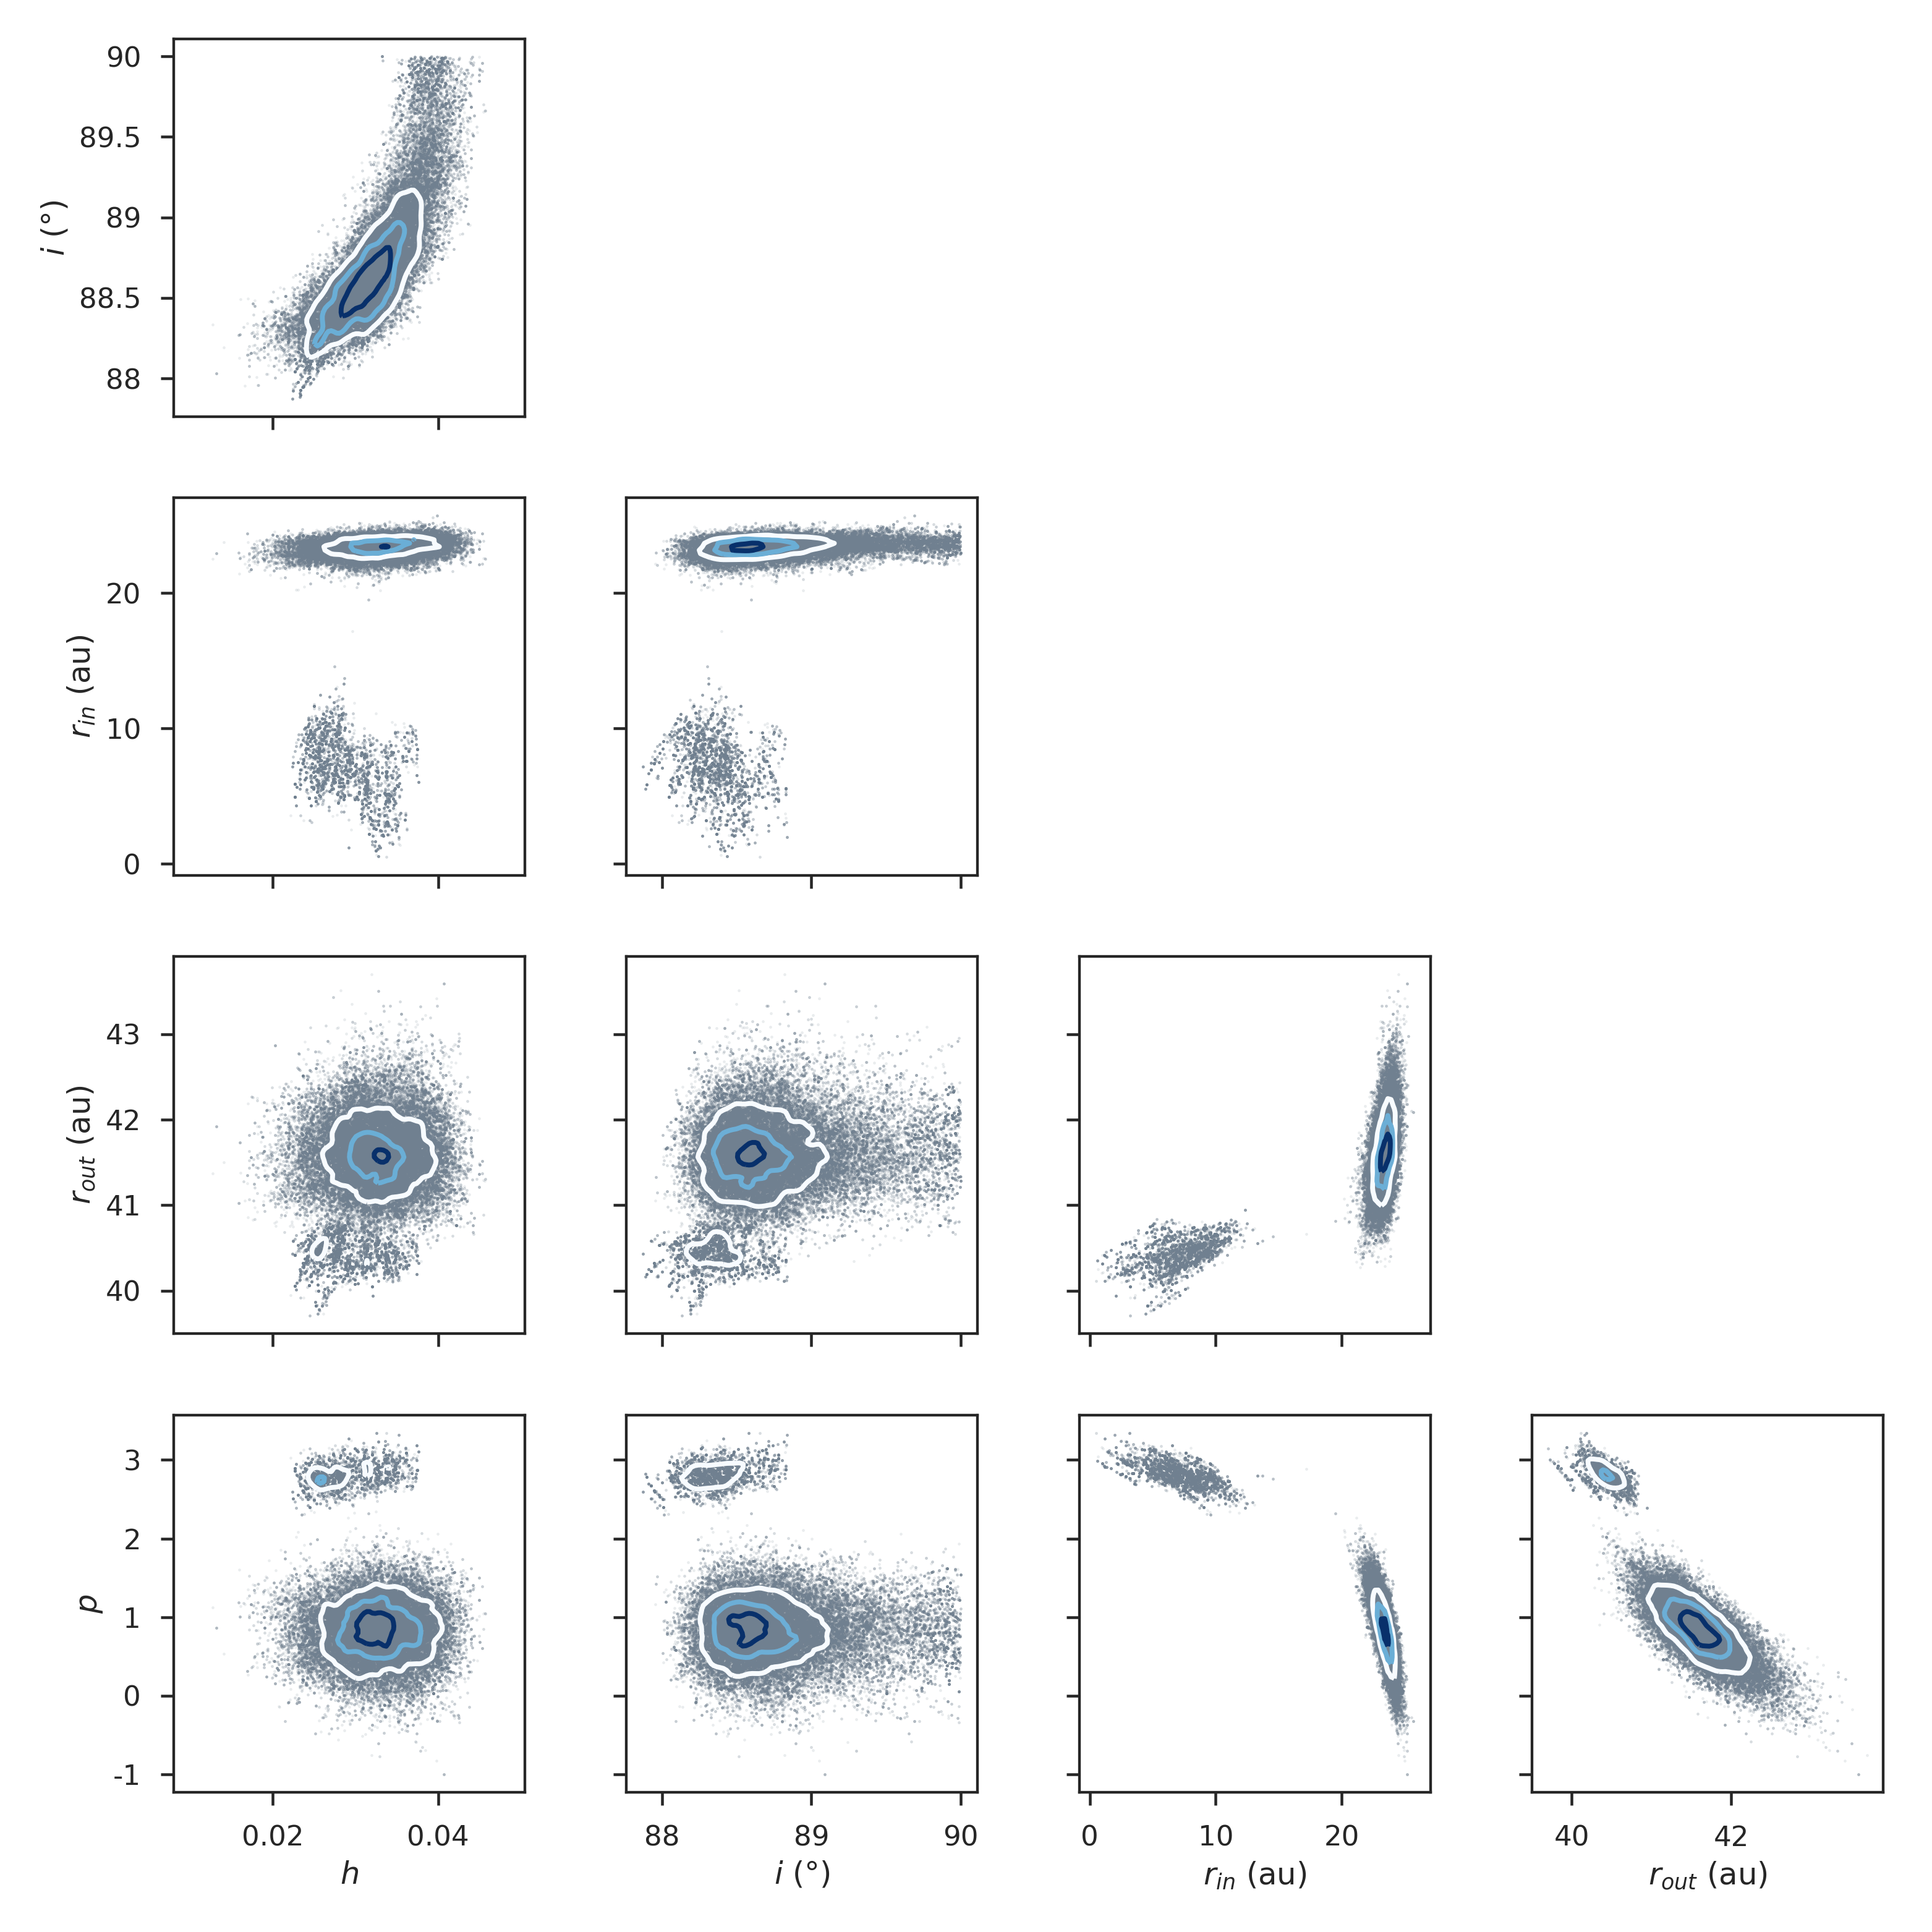
\includegraphics[width=0.9\linewidth]{../figures/degeneracy_corner}
  \caption{`Corner' plot showing degeneracies between a subset of the free parameters for the fiducial model.
  Two families of solutions are visible, and are most prominent in the $p$, $r_{in}$, and $r_{out}$ distributions.
  In addition, the two-dimensional slices through parameter space show limited degeneracies between radial structure, vertical structure, and viewing geometry.}
  \label{fig: degeneracies}
\end{figure}

\section{Investigating Radial Structure}
\label{section: radial analysis}

Marginalized posterior probability distributions for the fiducial model parameters are shown in Figure \ref{fig: kde}.
While the majority of the distributions are Gaussian, the three parameters that determine the radial structure of the disk ($p$, $r_{in}$, and $r_{out}$) exhibit slight bimodality. 
All three parameters are degenerate as can be seen from the `corner' plot in Figure \ref{fig: degeneracies}; in fact, the bimodality of the three parameters is a result of the existence of two distinct families of solutions in parameter space.
While the fiducial best-fit model has $p=0.8$, $r_{in}=\SI{24.0}{au}$, and $r_{out}=\SI{42.3}{au}$, a lower-likelihood family of solutions can clearly be seen in Figure \ref{fig: degeneracies}. The highest-likelihood model associated with this family has $p = 2.8$, $r_{in} = \SI{5.2}{au}$, and $r_{out} = \SI{41.0}{au}$.
More generally, mild degeneracies between the parameters determining vertical structure, radial  structure, and viewing geometry are visible, but the aspect ratio $h$ remains relatively uncorrelated with other aspects of AU Mic's structure.

The fiducial best-fit model image and residuals found in Figure \ref{fig: fiducial} provide further information as to the cause of the bimodal posterior distribution.
As can be seen from the residual map, the outer regions of the disk are reproduced well by the model; however $3\sigma$ residuals remain at the location of the star, as well as at symmetric positions at a separation of $\sim \SI{10}{au}$ on either side of the star. 
We note the symmetric residuals share the locations of the local intensity maxima described in \S \ref{chapter: results}. 
The convergence of these features leads us to consider the possibility of either a dust density enhancement (a ring) or reduction (a gap) in the inner regions of the disk. 
As a gap/ring would cause the radial surface brightness profile of the disk to deviate from that given by the simple power law used in our modeling, it could explain the bimodality in the posterior distributions of the parameters governing disk radial structure.

\begin{figure}
  \centering
  
  \subfloat[Fiducial run best-fit model and residuals.]{%
    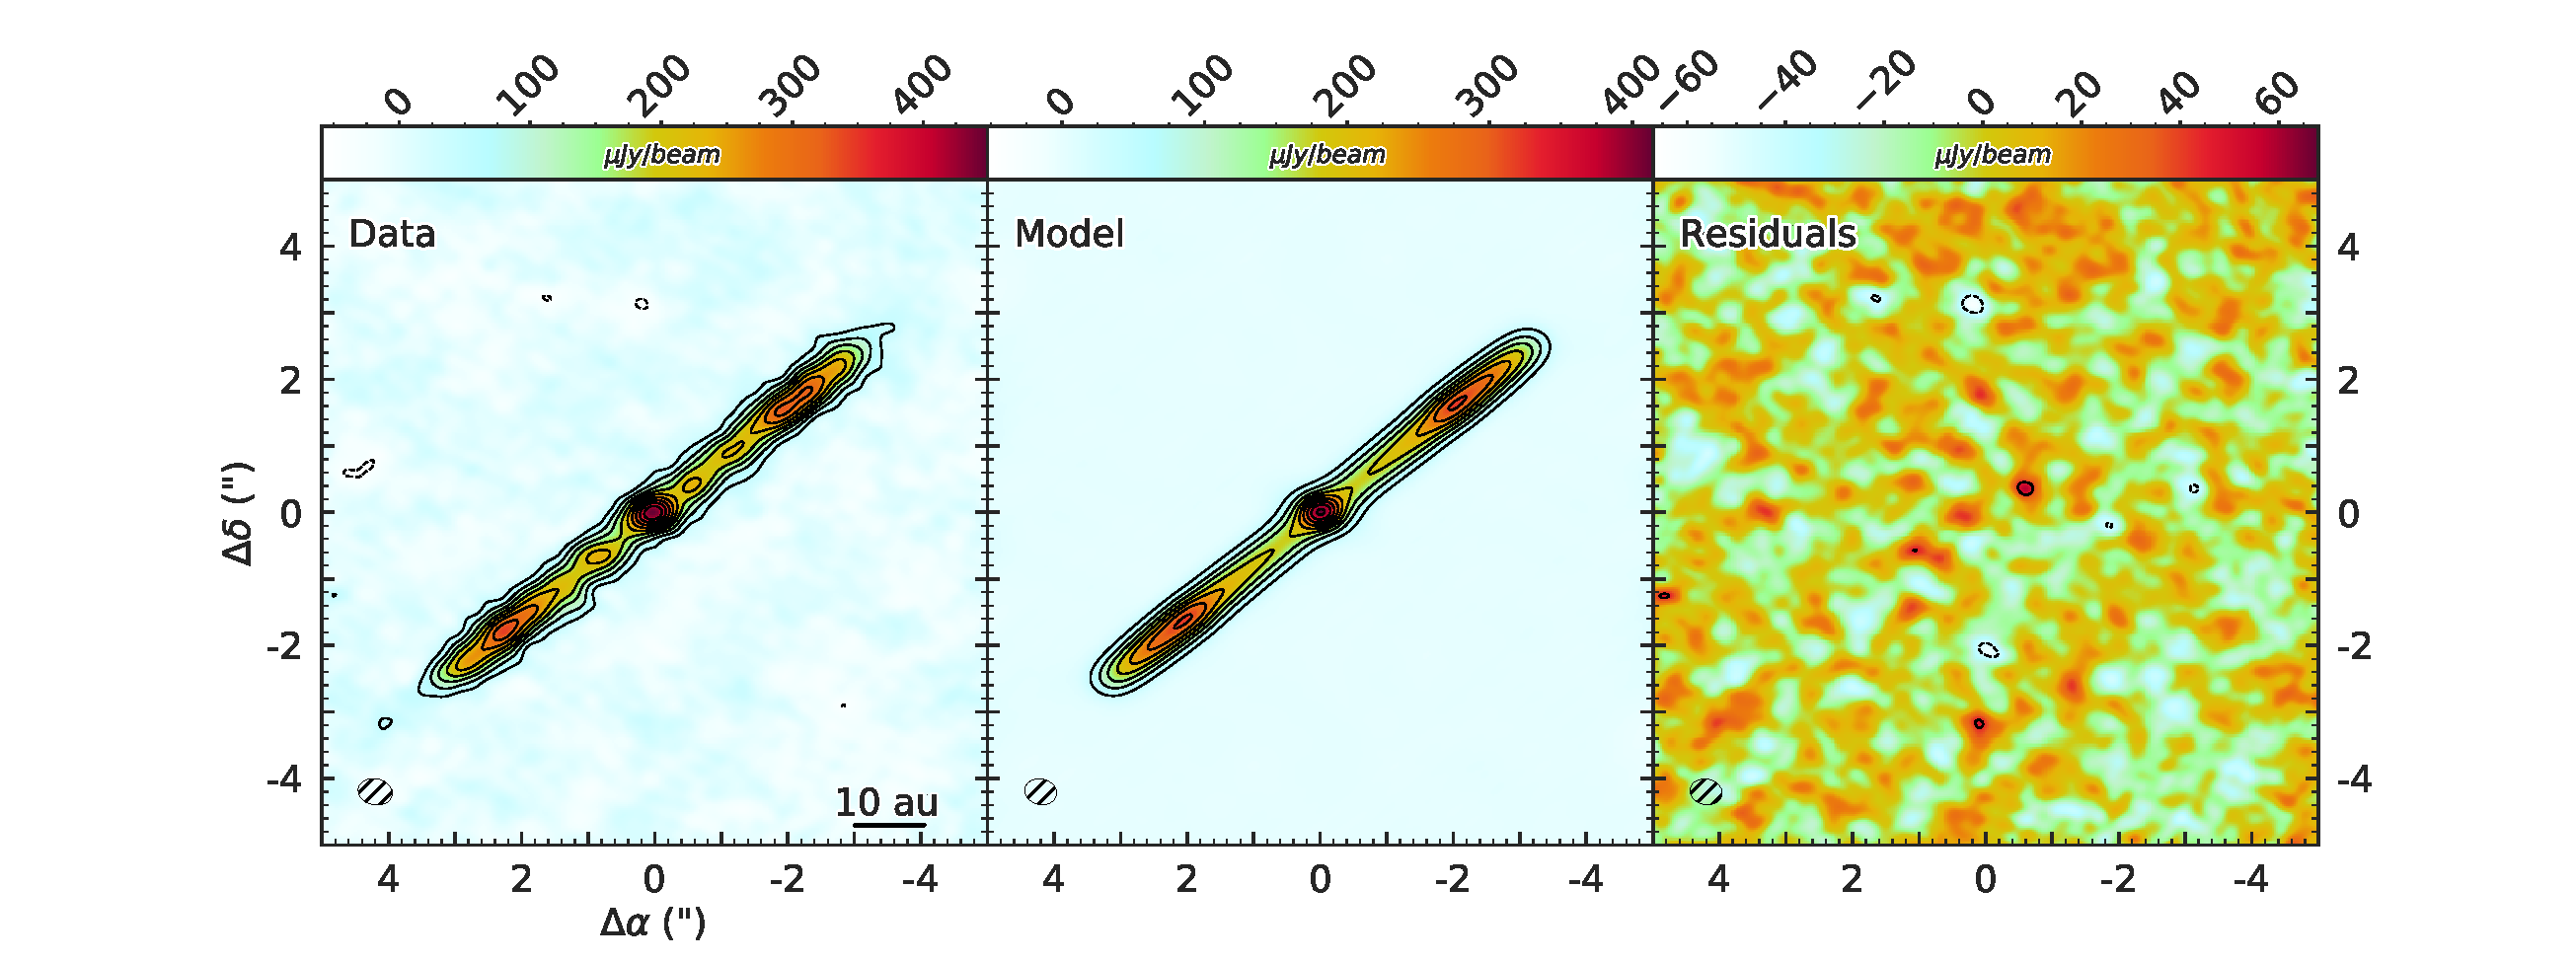
\includegraphics[width=0.77\linewidth]{../figures/fiducial_best_fit}%
    \label{fig: fiducial}%
    }\qquad
    
  \subfloat[Ring run best-fit model and residuals.]{%
    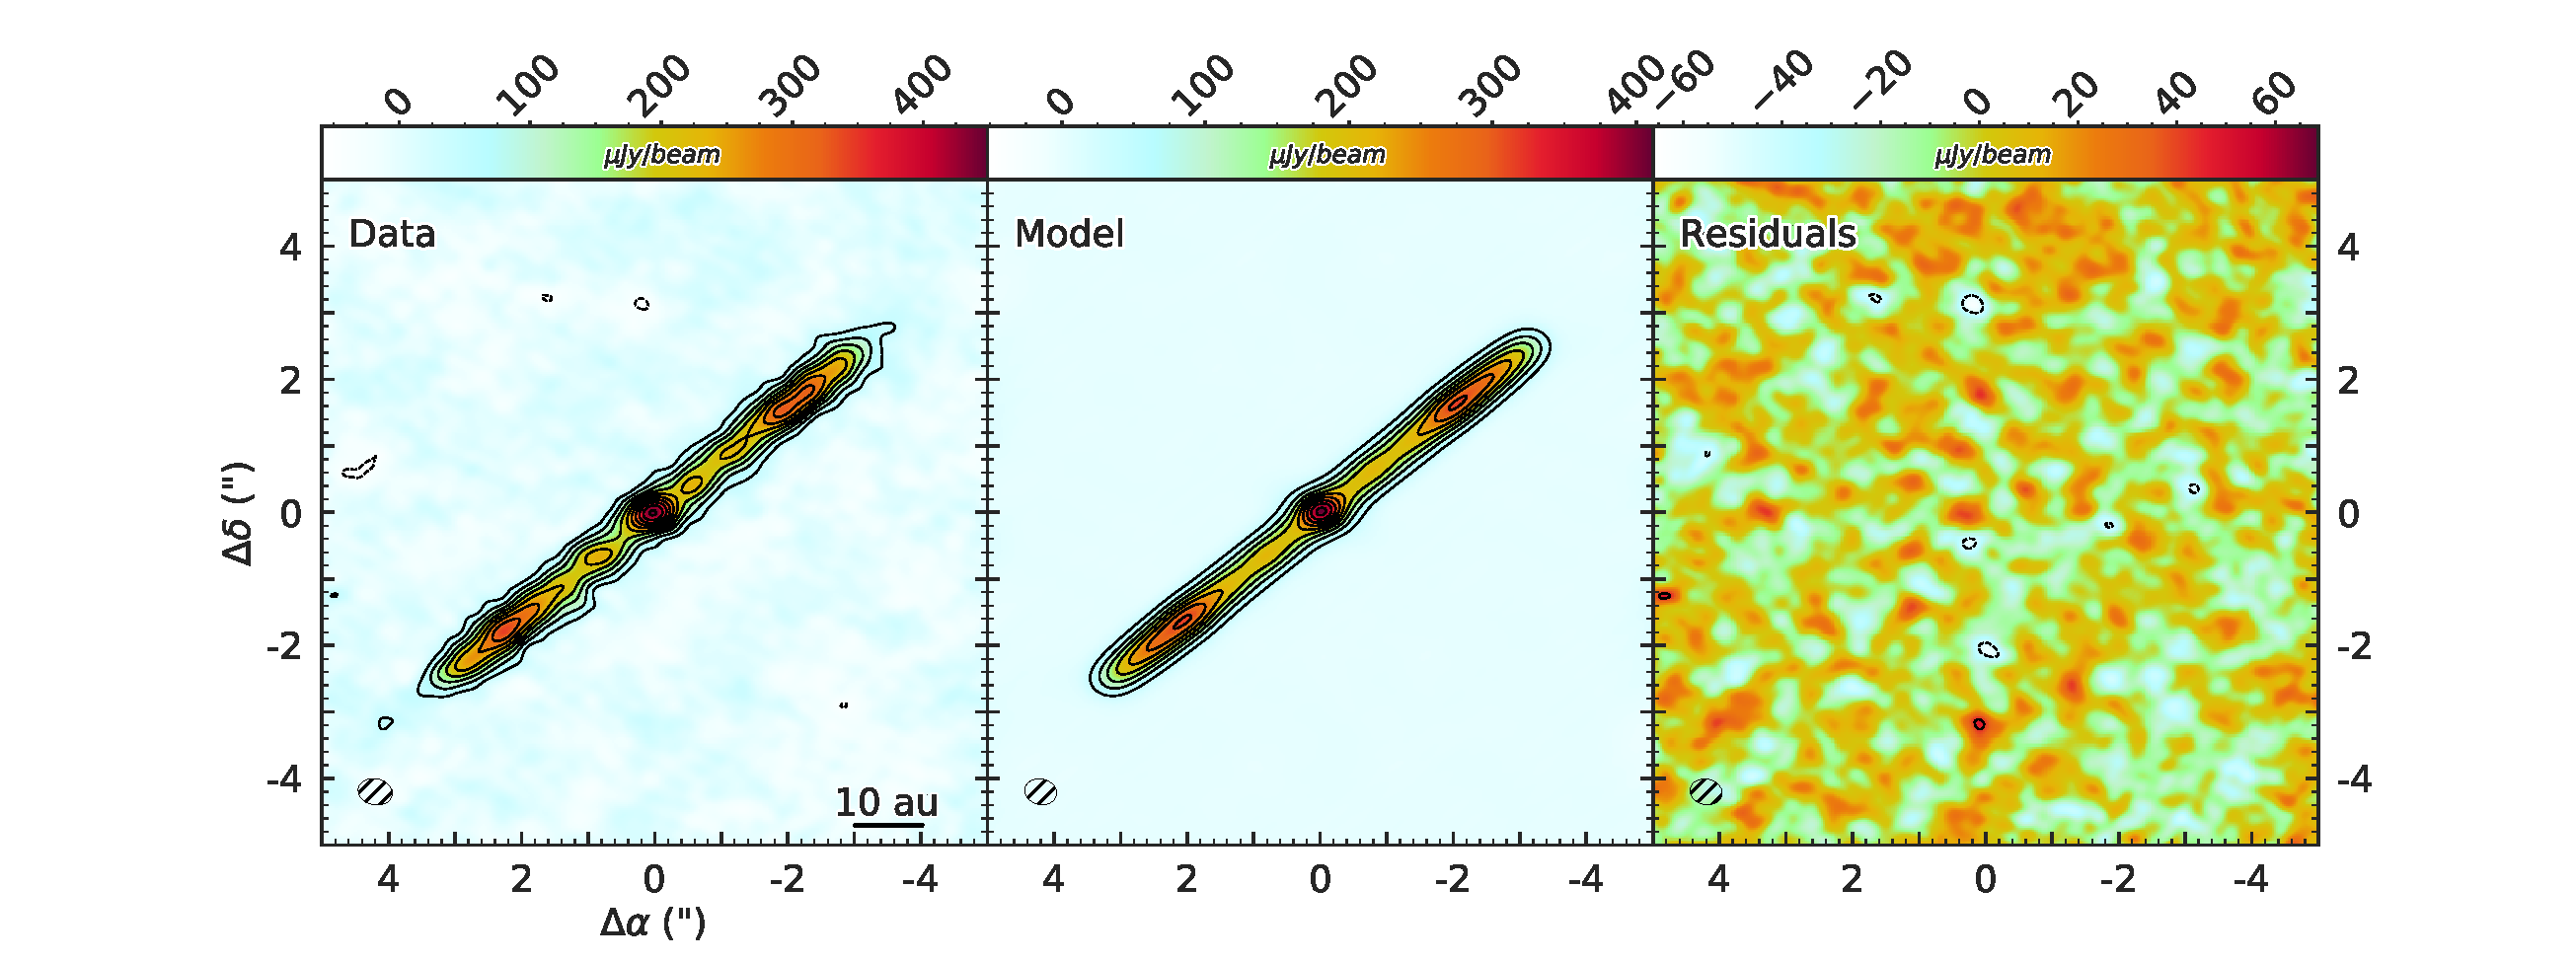
\includegraphics[width=0.77\linewidth]{../figures/annulus_best_fit}%
    \label{fig: ring}%
    }\qquad

  \subfloat['Skinny' disk run best-fit model and residuals.]{%
    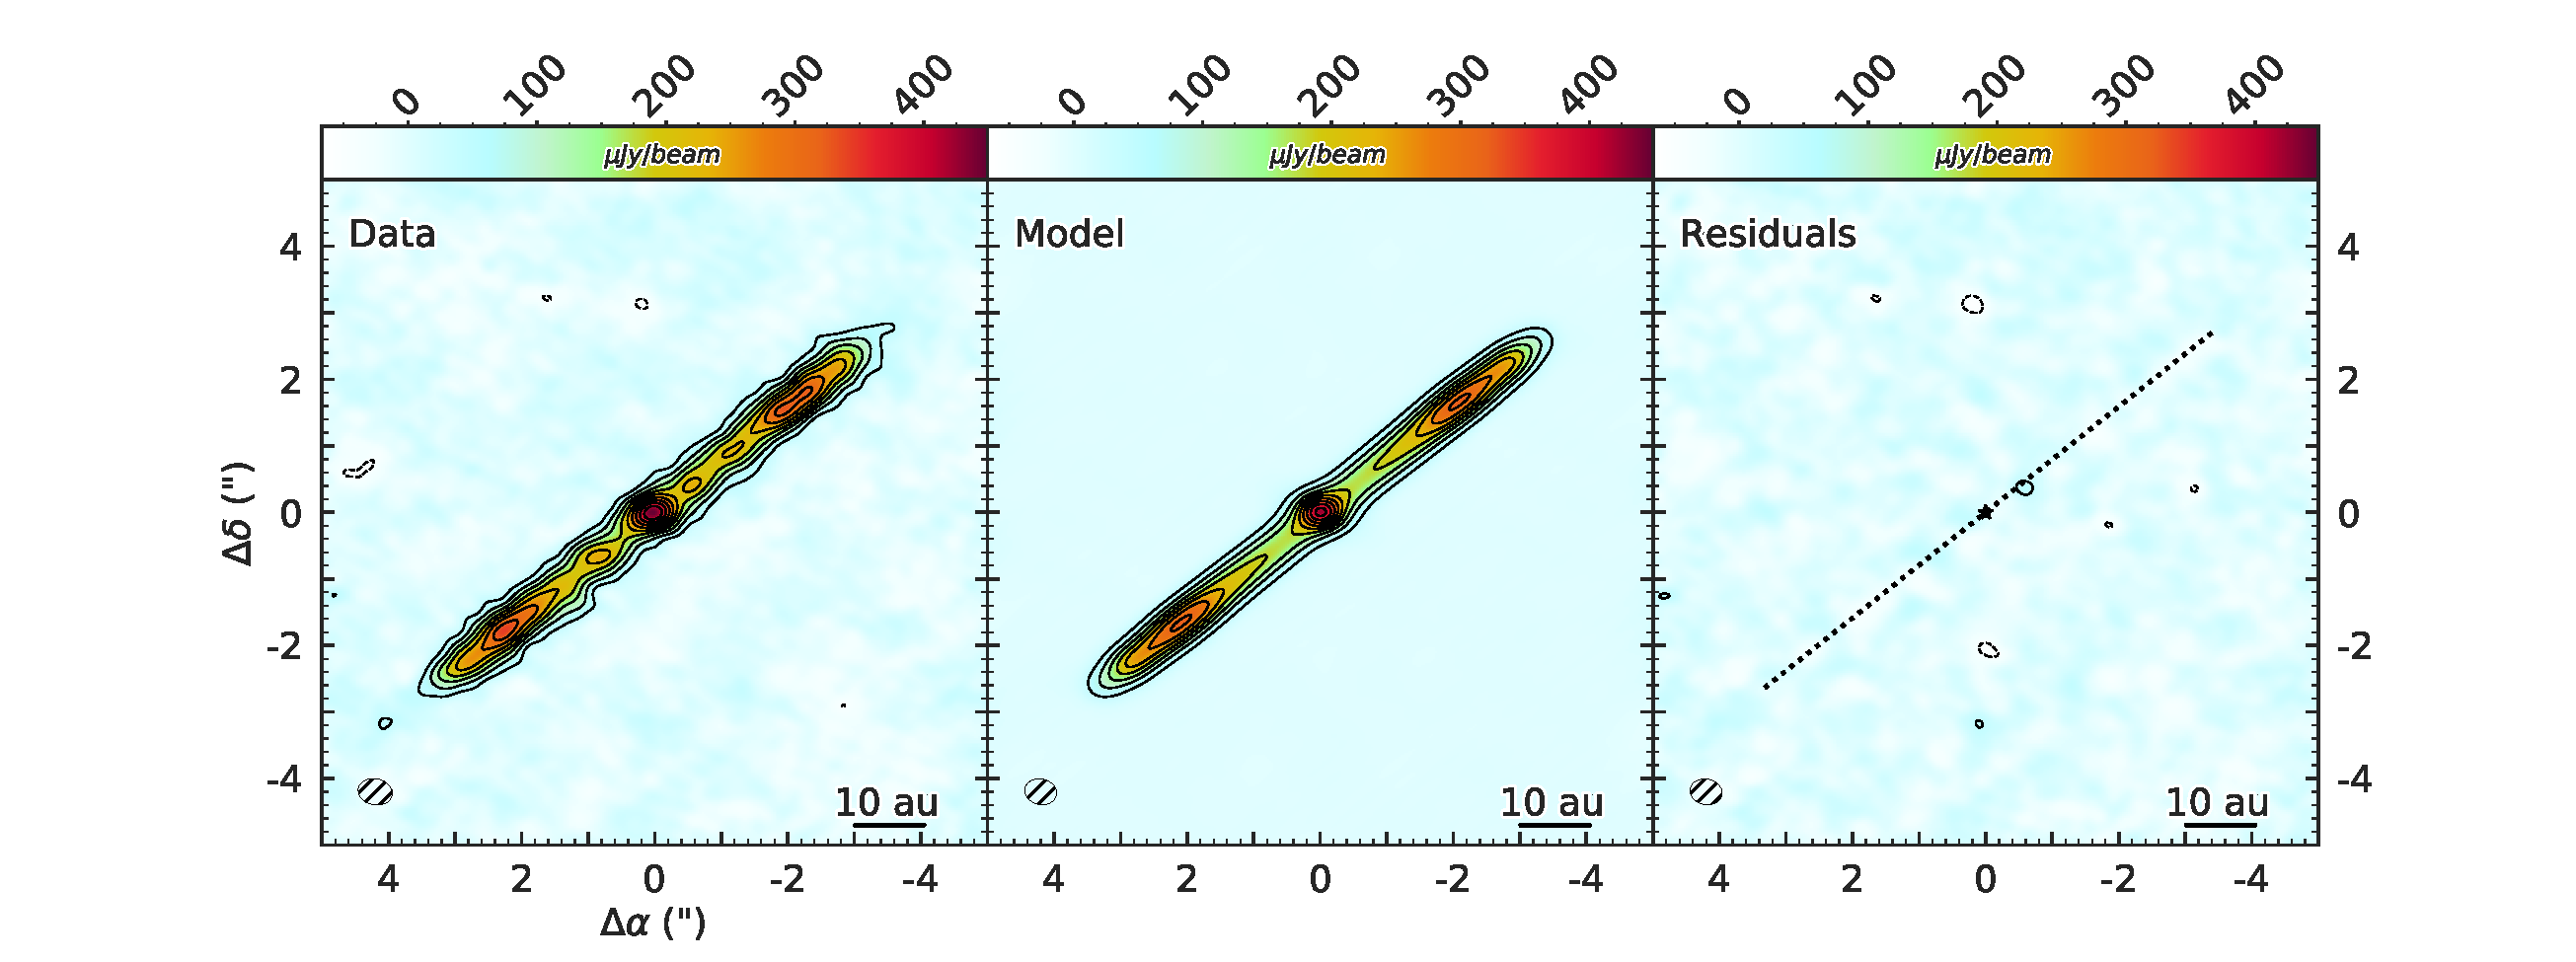
\includegraphics[width=0.77\linewidth]{../figures/skinny_best_fit}%
    \label{fig: skinny}%
    }\qquad
    
  \caption{Best-fit model image and residuals, sampled at the spatial frequencies of the ALMA data and cleaned using natural weighting. 
  Contours are integer multiples of the ALMA data $3\sigma$ confidence level. 
  For the fiducial model (a), $3\sigma$ residuals can clearly be seen at the location of the star and at symmetric positions $\sim \SI{10}{au}$ from the star. 
  Adding an additional ring of dust to the model (b) reduces these residuals by $\sim 25 \%$, but statistical analysis indicates that best-fit ring model does not conclusively describe the data better than the fiducial model.
  Fixing the scale height well below ALMA's resolution limits (c) results in a less statistically significant model, especially in the outer regions of the disk where ALMA is sensitive to the vertical structure of the disk.}
\end{figure}


We first explored the effects of adding a gap  to the inner regions of the disk. 
The gap inner and outer radii were left as free parameters and the dust density within the gap was set to zero.
The gap consistently converged to regions where the dust density was already zero (interior to the disk inner radius or exterior to the disk outer radius); we take this as evidence that the data is not well characterized by a gap.
As a next step, we experimented with adding a ring to the disk. 
The ring inner radius $r_{ring}$ was once again left as a free parameter and the ring width was fixed to \SI{0.3}{au}.
The ring was also characterized by a dust mass $M_{ring}$, which was evenly distributed across the radial extent of the ring. 
As can be seen in Figure \ref{fig: ring} this parameterization was better able to reproduce the `bump' in the radial surface brightness profile at $r \sim \SI{10}{au}$, reducing the best-fit model residuals by $\sim 25 \%$. 
However, $2 \sigma$ residuals are still present at the location of the bumps; the ring model's failure to accurately reproduce these features could be explained by the fact that the two local intensity maxima are not perfectly symmetric about the star. 
Image domain analysis indicates that the bump to the SE has a separation of $\sim \SI{11}{au}$, while the NW bump has a separation of $\sim \SI{8}{au}$  (Figure \ref{fig: boccaletti}). 
This discrepancy could be explained if the hypothetical ring were eccentric.

The median values and best-fit model parameters for the fiducial and ring parameterizations can be found in Table \ref{tab: params}. 
We use both the AICc, a form of the Aikake Information Criterion (AIC) corrected for finite datasets, and the Bayesian Information Criterion (BIC) to compare goodness of fit between models with different numbers of free parameters.  
The best-fit ring model is preferred to the fiducial model with $3.72 \sigma$ confidence on the AICc; conversely, the fiducial model is preferred to the ring model on the BIC with $\Delta \text{BIC} = 4.26$.
As such, we are not able to conclusively confirm the presence of an additional ring of mm dust grains in the AU Mic disk.
A model with a single $F_\star$ across all three dates was also investigated, but did not reproduce the data to the same degree of accuracy as the fiducial model.
Significant residuals were visible at the location of the star, and analysis using the AICc indicates that a stellar flux varying by more than a factor of 2 over a period of months to years is preferred with a $7.3 \sigma$ confidence interval.

\begin{table}
  \centering
  \caption{MCMC Fitting Results}
  \label{tab: params}
  \renewcommand{\arraystretch}{1.2}
  \begin{tabular}{lrrrr}
  \toprule
    \multirow{2}{*}{Parameter} & \multicolumn{2}{c}{Fiducial} & \multicolumn{2}{c}{Disk + Ring} \\ 
    \cmidrule(lr){2-3} \cmidrule(lr){4-5} 
    & Median & Best Fit & Median & Best Fit \\
  \midrule
    $\log M$ (\si{M_\earth})   & $ -7.540 _{-0.006} ^{+0.006}$ & $-7.540$  & $-7.548  _{-0.007} ^{+0.007}$ & $-7.545$ \\
    $p$                        & $0.9     _{-0.4}   ^{+0.5}$   & $0.8$     & $0.8     _{-0.4}   ^{+0.6}$   & $0.9$     \\
    $h$                        & $0.031   _{-0.005} ^{+0.005}$ & $0.032$   & $0.027   _{-0.005} ^{+0.004}$ & $0.028$   \\
    $r_{in}$ (\si{au})         & $23.8    _{-0.9}   ^{ +0.6}$  & $24.0$    & $24.1    _{-0.9}   ^{+0.6}$   & $23.9$    \\
    $r_{out}$(\si{au})         & $42.3    _{-0.5}   ^{ +0.4}$  & $42.3$    & $42.3    _{-0.5}   ^{+0.4}$   & $42.4$    \\
    $i$ (\si{\degree})         & $88.6    _{-0.3}   ^{ +0.4}$  & $88.7$    & $88.27   _{-0.16}  ^{+0.22}$  & $88.3$    \\
    PA  (\si{\degree})         & $128.49  _{-0.07}  ^{+0.07}$  & $128.50$  & $128.50  _{-0.07}  ^{+0.07}$  & $128.48$  \\
    March $F_*$ (\si{\mu Jy})  & $390     _{-20}    ^{+20}$    & $390$     & $370     _{-20}    ^{+20}$    & $370$     \\
    August $F_*$ (\si{\mu Jy}) & $150     _{-30}    ^{+20}$    & $160$     & $150     _{-30}    ^{+20}$    & $140$     \\
    June $F_*$ (\si{\mu Jy})   & $220     _{-20}    ^{+20}$    & $220$     & $220     _{-20}    ^{+20}$    & $210$     \\
    $r_{ring}$ (\si{au})       &                               &           & $11.9    _{-1.8}   ^{+1.7}$   & $10.8$      \\
    $M_{ring}$ ($\si{M_\earth} \times 10^{-4})$  &             &           & $1.8     _{-0.7}   ^{+0.5}$   & $1.7$     \\
    $\ln$ Likelihood           & $-313087 _{-4}     ^{+2}$     & $-313082$ & $-313077 _{-5}     ^{+2}$     & $-313072$ \\
  \bottomrule
  \end{tabular}
\end{table}


\section{Investigating Vertical Structure}
\label{section: vertical analysis}

The posterior distribution for the aspect ratio $h$ suggests that the data are capable of measuring AU Mic's scale height despite the mild degeneracy between aspect ratio and other parameters like the radial structure and viewing geometry.  
Even when marginalized over these other parameters, the posterior distribution indicates a measured value of $h=\num{0.031 \pm 0.005}$, which translates to a $\sim 6 \sigma$ measurement of the scale height rather than an upper limit.
At the $\sim \SI{40}{au}$ outer edge of the disk, this aspect ratio implies a vertical scale height of \SI{1.2 \pm 0.2}{au}. 
The corresponding disk FWHM is \SI{2.8 \pm 0.5}{au}, consistent with an image-domain FWHM of $\sim \SI{3}{au}$ estimated from Figure \ref{fig: boccaletti}.
To verify that we in fact measured the scale height, we investigate a model parameterization in which the scale height is set to a value well below ALMA's resolution limits.
The aspect ratio is fixed at a value of $0.003$, so that even at the outer edge of the disk the scale height is $\sim \SI{3}{\percent}$ of the beam size along the disk's vertical axis.
If the disk is in fact resolved, such a `skinny' disk model should perform significantly worse than the fiducial model.
The best-fit model image and residuals are shown in Figure \ref{fig: skinny}.
The skinny model results in a significantly poorer fit to the data than the fiducial model with variable aspect ratio, with the best fits differing at the $4.1\sigma$ level according to the AICc and by a value of 9.5 on the BIC.

The preferred disk FWHM is only $\sim 2/3$ the size of the combined-data beam projected onto the vertical axis of the disk.
While it may seem improbable that we measure a scale height below the image-domain spatial resolution of the combined data, our results can be explained by the following observations.
First, the beam size of the naturally weighted combined image ($\SI{0.52}{\arcsecond} \times \SI{0.39}{\arcsecond}$) is not wholly representative of the longest baselines in the data. 
The smallest naturally weighted beam FHWM from the three individual observations is \SI{0.30}{\arcsecond} (Table \ref{tab:observations}), while the spatial scale traced by the longest baseline is \SI{0.22}{\arcsecond}.
Second, the scale height $H$ refers to the disk height as measured from the midplane; the observable quantity that must be resolved in order to measure the scale height is actually the total vertical thickness $2H$.
Third, the scale height represents the standard deviation of a Gaussian distribution of dust particles that in fact reaches well beyond the extent of the scale height.
For example, considering that the peak SNR of the data is $\sim 23$ and that the vertical distribution of dust is assumed to be Gaussian, the SNR should remain above 3 over a total vertical extent of \SI{3.8}{au}. 
The combination of these factors indicates that it is plausible that we are able to detect a scale height smaller than the resolution of the image-domain data.


\clearpage
\chapter{Discussion}
\label{chapter: discussion}

Parametric modeling suggests that AU Mic's debris disk is nearly edge on, exhibits an increasing surface density with radius until $\sim\SI{42}{au}$, and reaches a maximum scale height of $\sim\SI{1.2}{au}$.
There is also marginal evidence for an additional annulus of dust at $r \sim \SI{10}{au}$.
Here we compare the results of our analysis with previous studies of AU Mic's debris disk.

The geometric properties of the disk inferred from our modeling agree well with the literature. 
Our median inclination of $\ang[angle-symbol-over-decimal]{88.6}^{+0.4}_{-0.3}$ is consistent with previous estimates of the disk's inclination within uncertainties \citep{metchev05,krist05}.
The median PA of $\ang[angle-symbol-over-decimal]{128.49} \pm 0.07$ falls within uncertainties of measurements by \cite{macgregor13} and \cite{krist05}; however, the limb-averaged PA interior to \SI{50}{au} from \cite{metchev05} is $\ang[angle-symbol-over-decimal]{129.8} \pm 0.2$, and \cite{schneider14} report an optical-wavelength PA of $\ang[angle-symbol-over-decimal]{127.8} \pm 0.2$ between \SIrange{50}{100}{au}.
The preferred dust mass (\SI{0.01}{M_\earth}) is identical to the value derived from resolved \SI{1.3}{mm} imaging by \cite{macgregor13} and from low-resolution \SI{850}{\mu m} imaging by \cite{matthews15}; the latter quote a 20\% uncertainty.
Similarly, \cite{liu04} report \SI{0.011}{M_\earth} from unresolved \SI{850}{\mu m} observations.
\cite{strubbe&chiang06} calculate \SI{0.01}{M_\earth} by deriving a steady-state collisional cascade grain size distribution and fitting the disk's surface brightness and thermal spectrum to $V$- and $H$-band HST observations.

Our analysis indicates with high confidence that AU Mic exhibited long-term millimeter variability over the $\sim \SI{1.5}{yr}$ observation period; this phenomenon is distinct from the \SI{6}{minute} flare that occurred during the June observations.
The stellar fluxes preferred by our modeling vary by more than a factor of two, and are comparable to \cite{macgregor13}'s best-fit flux of \SI{320 \pm 60}{\mu Jy}.
Pre-main sequence stars have been shown to exhibit both short- and long-term variability in the radio \citep{forbrich17,rivilla15}, but there is little evidence for such behavior among low-mass main sequence stars.
Simulations of radio emission from low-mass stars allow for variability of more than a factor of two over the entire longitudinal extent of a star \citep{llama18}; it may be that different longitudinal regions of AU Mic were facing Earth during the three observations.


\section{Radial Structure}
\label{section: radial discussion}

\begin{figure}
  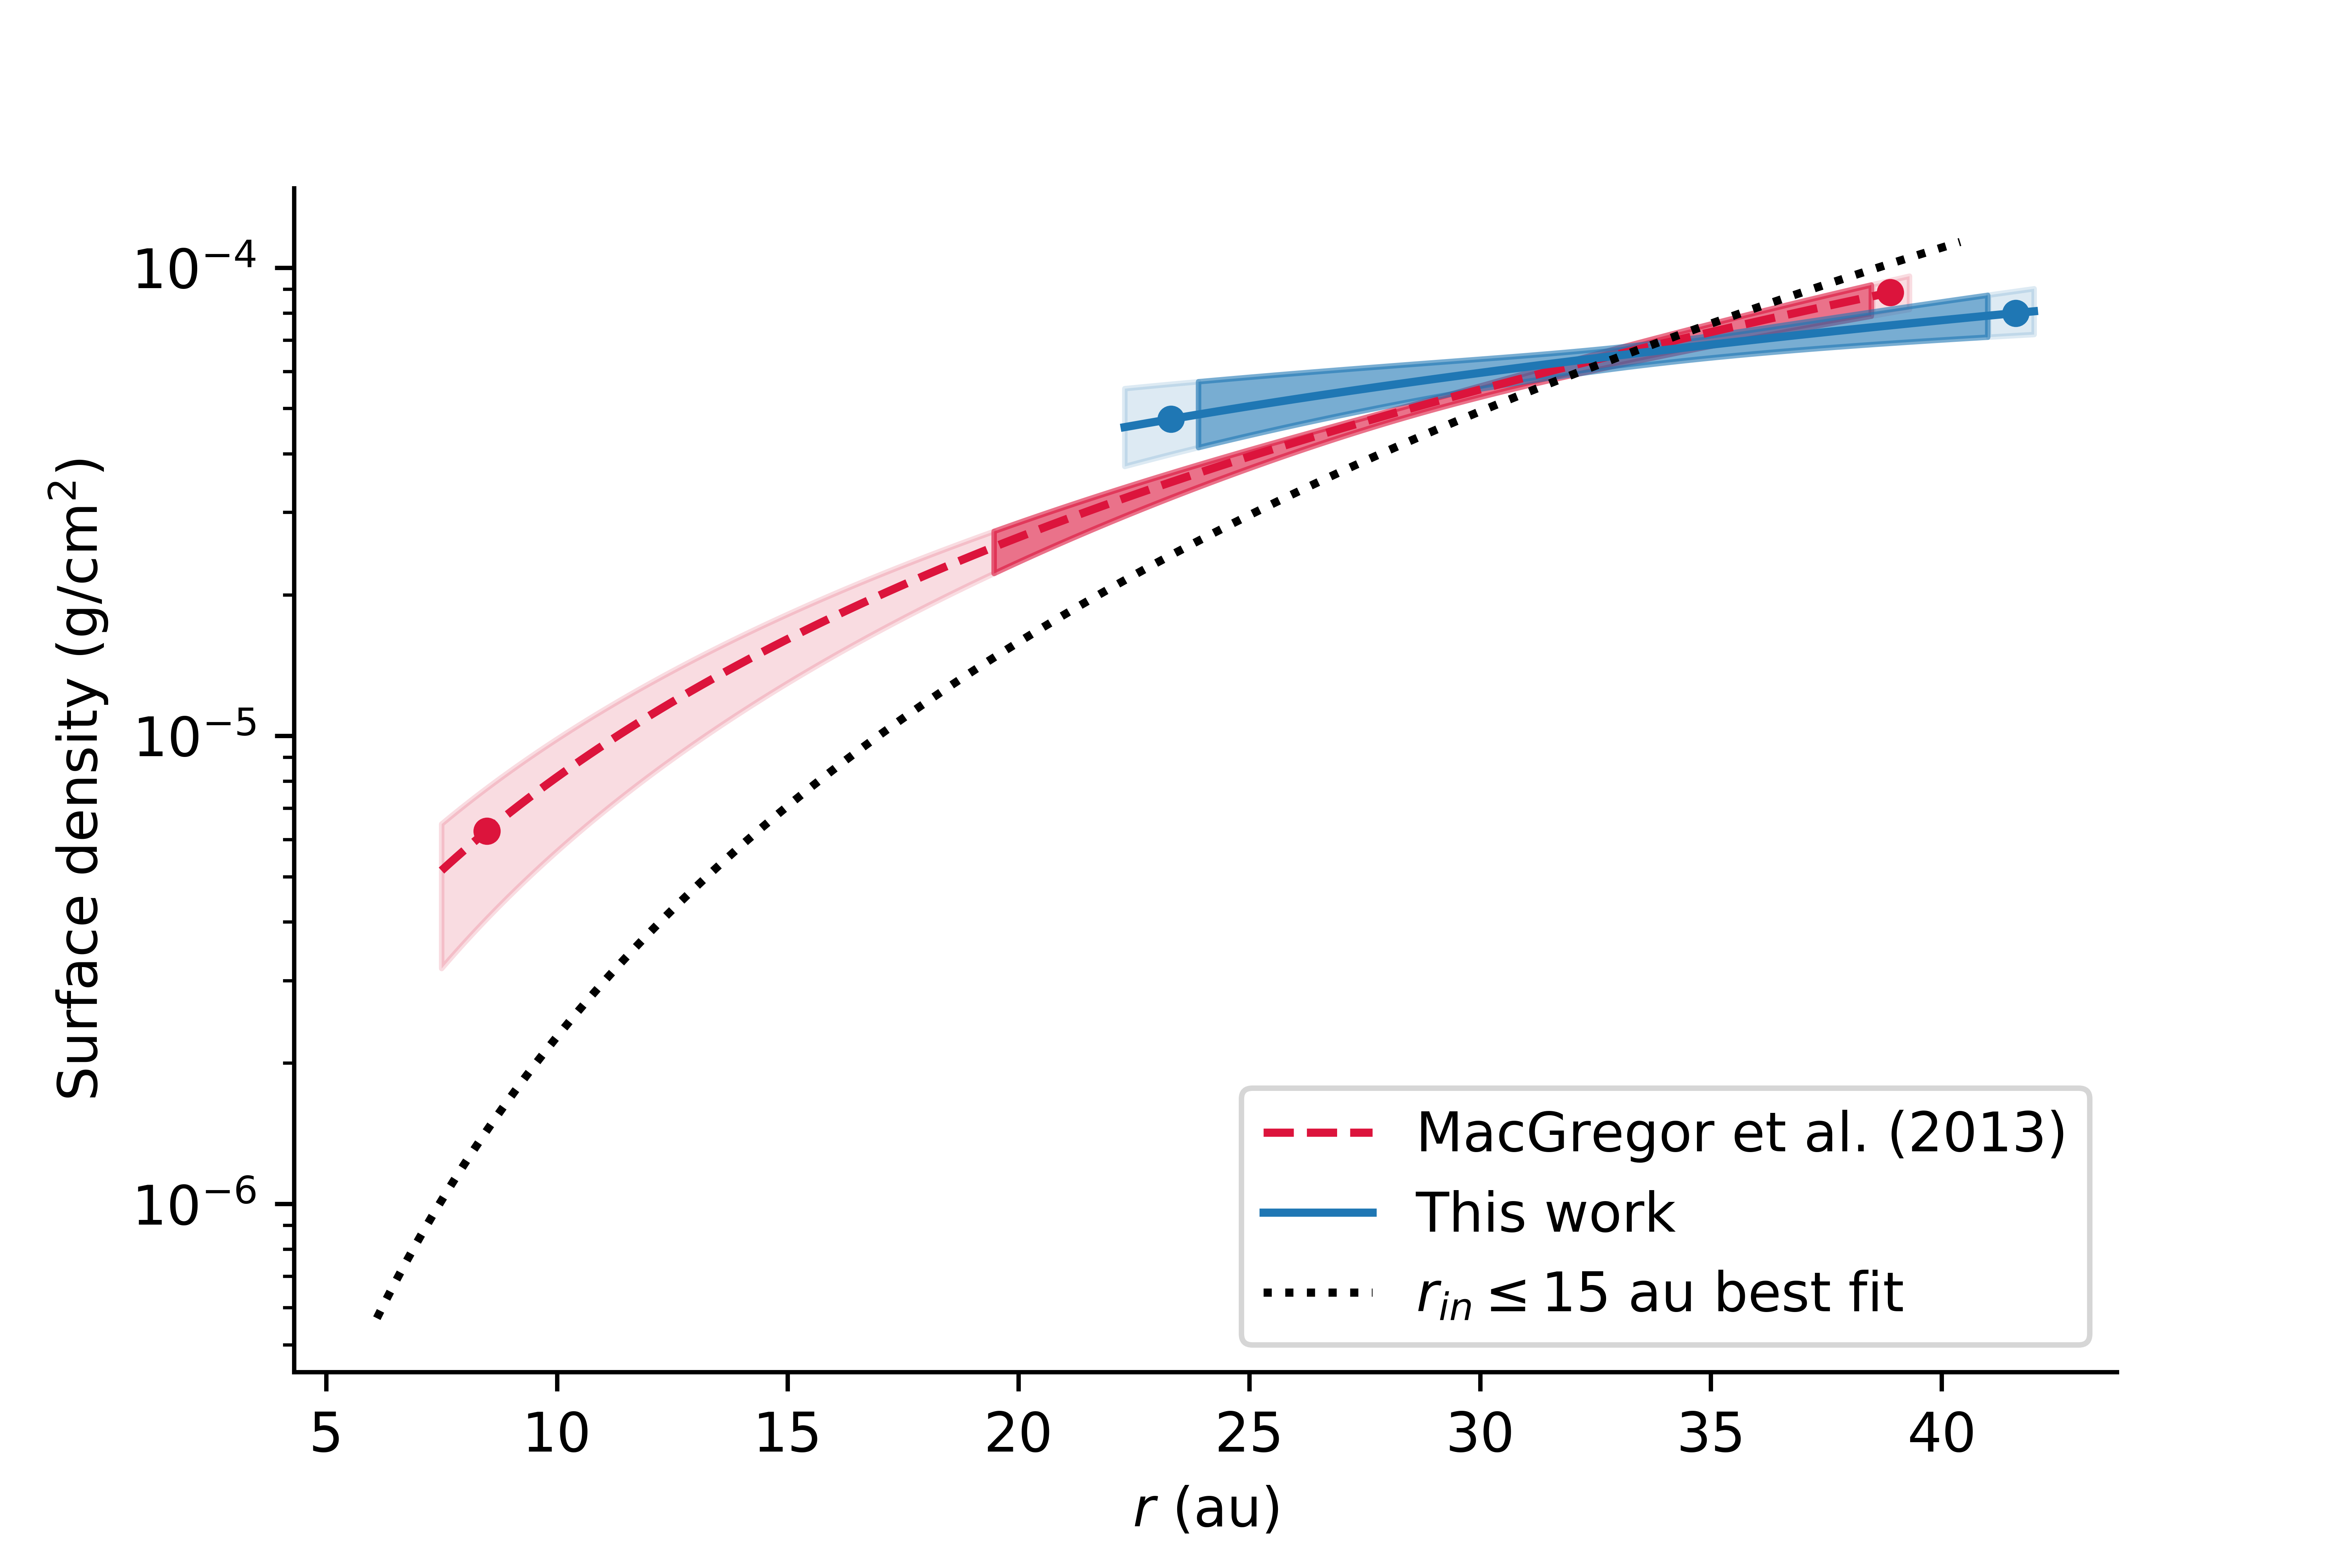
\includegraphics[width=\linewidth]{../figures/surface_density}
  \caption{
    Comparison between the best-fit surface density profiles obtained in \cite{macgregor13} (solid red line) and this work (dashed blue line).
    Also included is the best-fit surface density profile associated with the lower-likelihood family of solutions (dotted black line).
    The vertical extent of the shaded regions marks $1\sigma$ confidence intervals on the surface density. 
    The points designate the best-fit inner and outer radii for each model, and the horizontal extent of the more transparent shaded regions show $1 \sigma$ confidence intervals on the inner and outer radii.
    Not included in the uncertainties are the 10\% flux uncertainties of each observation.
    }
  \label{fig surface_density}
\end{figure}

Modeling of the radial structure discussed in \S \ref{section: radial analysis} is broadly consistent with the previous analysis of millimeter wavelength emission from the disk performed by \cite{macgregor13} as can be seen in Figure \ref{fig surface_density}. 
However, the factor of $\sim 2$ increase in spatial resolution introduces additional interpretive complexities when comparing the results.
While our outer radius is only \SI{2}{au} larger than than the previously reported value of \SI{40.3}{au} (confidence intervals are $\sim \SI{0.4}{au}$ for both measurements), things become more complicated when considering the inner radius $r_{in}$ and surface brightness power law index $p$.
In contrast to $r_{in} = 23.8_{-0.9}^{ +0.6}$ \si{au} preferred by our MCMC analysis, \cite{macgregor13} report $8.8_{-1.0} ^{+11.0}$ \si{au}.
Neither parameter is well constrained: the authors report a $3 \sigma$ upper limit of \SI{21}{au}, whereas conversely we find a $2 \sigma$ lower limit of $\sim \SI{1}{au}$.
Similar discrepancies arise in the posterior distribution for $p$, which is degenerate with $r_{in}$.
While \cite{macgregor13} finds $p=2.32_{-0.31}^{+0.21}$, we recover a median value of $p=0.9_{-0.4}^{+0.5}$.
In our analysis, the uncertainties in these two parameters arise from the existence of two families of solutions: one at $r_{in} \sim \SI{23}{au},\ r_{out} \sim \SI{42}{au},\ p \sim 0.8$ and another at $r_{in} \sim \SI{5}{au},\ r_{out} \sim \SI{41}{au},\ p \sim 2.8$ (Figure \ref{fig surface_density}).
The latter family, which has a lower likelihood, is probably associated with the local intensity maxima on either of the star examined in \S \ref{chapter: analysis}.
Our exploratory modeling of these features raises the possibility of an annulus of dust interior to the main disk---if such an annulus does exist, the $\sim 2$ times lower resolution observations from \cite{macgregor13} would probably not have been able to distinguish the annulus emission from that of the main disk.
In fact, an unresolved annulus would likely bias the inner radius preferred by the authors' modeling towards smaller values and could account for the differences in our characterization of the radial structure.

While the annulus model provides only a marginally significantly improved fit to the data, previous observations spanning a wide range of wavelengths have recovered surface brightness enhancements at the same projected stellocentric separation ($\sim~\SI{10}{au}$) as the hypothetical annulus.
A local maximum is present to the SE of the star at this separation in lower-resolution ALMA observations by \cite{macgregor13}, and there is a suggestive peak in the noise on the opposite side of the star as well.
Although these surface brightness enhancements do not attain $3 \sigma$ significance after subtraction of an axisymmetric model, the independent detection of these features in both data sets suggests that they may be real.  
\cite{schneider14} also observe an optical-wavelength `bump' $\sim \SI{13}{au}$ SE of the star and slightly elevated from the disk midplane (i.e. to the NE).
No matching surface brightness enhancement is observed on the NW side of the disk, which is obscured by the STIS occulting wedge for $r \lesssim \SI{12}{au}$.
On the other hand, the scattered light emission on the NW side is not symmetric about the midplane and the authors tentatively identify a warp below the midplane extending to a distance of $\sim \SI{45}{au}$ from the star.
They note that these features may share a common causality, and posit that dust orbits in the inner disk are non-coplanar with those found at larger separations.

Near-infrared GPI obsevations presented in \cite{wang15} further corroborate the presence of a `bump' to the SE, characterized by a FWHM roughly triple the FWHM at an equivalent separation on the NW side of the disk. 
No features are detected at a corresponding separation to the NW.
Figure 4 of \cite{wang15} shows a composite map of the bump as seen by GPI, STIS, and ALMA; the common location of the bump in both scattered light and mm observations would indicate that the mm- and micron-sized grains are cospatial.
The micron-sized grains traced by scattered light are thought to be mostly confined to a narrow `birth ring' at $\sim \SI{40}{au}$ \citep{strubbe&chiang06}. 
Thus, if the millimeter bump visible in both this work and in \cite{macgregor13} is indeed cospatial with the scattered light bump, it would suggest that the true stellocentric separation of of the millimeter feature is $\sim \SI{40}{au}$ and that its apparent stellocentric separation of $\sim \SI{10}{au}$ is due to projection effects.

\section{Vertical Structure}
\label{section: vertical discussion}

As discussed in \S \ref{section: vertical analysis}, our MCMC analysis yields a median aspect ratio of \linebreak $h~=~\num{0.031 \pm 0.005}$; at a reference point of \SI{40}{au}, this translates to a vertical scale height $H = \SI{1.2 \pm 0.2}{au}$.
This measurement is marginally consistent with values cited in the literature, ranging from roughly \SIrange{0.6}{2}{au} and derived from observations spanning the optical to the sub-millimeter.
\cite{schuppler17} place an upper limit of 0.05 on the \SI{1.3}{mm} opening angle (equivalent to the aspect ratio for small angles) by extracting the image-domain vertical profile from \cite{macgregor13}'s vertically unresolved ALMA observations, and estimate a visible-wavelength opening angle of 0.03 by reading off the vertical scale height from \cite{schneider14}'s STIS image of the disk.
\cite{metchev05} approximate a $H$-band Keck FWHM of $\sim \SI{4}{au}$ at a separation of \SI{40}{au};
\cite{krist05} fit a vertical Lorentzian profile to multicolor HST observations of the disk and find the FWHM interior to \SI{50}{au} to fall between \SIlist{2.5;3.5}{au}.

Because the measurements quoted above are determined from the observed vertical thickness of AU Mic's disk, they can be affected by the radial structure and viewing geometry of the disk as well as scattering effects. 
As such, parametric modeling provides a more reliable way to assess AU Mic's vertical structure.
\cite{krist05} report a FWHM between \SIlist{1.73;1.74}{au} at a separation of \SI{20}{au} from three-dimensional scattering models.
Collisional modeling can also be used to learn about AU Mic's vertical structure: collisional velocities---and thus dust production---are affected by the maximum eccentricity of planetesimal bodies $e_{max}$, which in turn can be related to the disk vertical stucture (see \S \ref{inferring mass} below). 
\cite{schuppler17} perform such modeling constrained by photometric observations spanning visible to millimeter wavelengths and quote a reference model opening angle of 0.015.
The authors go on to note that an opening angle of 0.005 better reproduces the disk spectral energy distribution (SED) in the long-wavelength regime beyond \SI{100}{\mu m}, but is unable to reproduce flux measurements for $\lambda \leq \SI{70}{\mu m}$.

In sum, estimates of AU Mic's vertical structure vary widely depending on the wavelength of observation, the techniques used, and the assumptions made.
Rigorous comparison between measurements in the literature is difficult---for example, \cite{krist05} assume a flared vertical profile while other authors use a linear parameterization for the scale height.
Nevertheless, some general statements may be made.
Values determined from optical and near-infrared observations range from roughly $H = \SI{1.2}{au}$ to \SI{2}{au} at a radius of \SI{40}{au}, while the values determined at least in part from mm observations range from $H = \SI{0.6}{au}$ to \SI{2}{au}, the latter being an upper limit. 
Estimates based on millimeter observations (including this work) tend to be smaller than those derived from shorter-wavelength observations, although the two wavelength regimes do not provide radically different values.

It is not unexpected that optical and infrared measurements of the scale height would exceed millimeter-wavelength estimates.
\cite{thebault09} suggests that the smaller grains traced by short-wavelength observations can be placed on inclined orbits by radiation pressure (and to first order, disk winds) even in the absence of large bodies dynamically stirring the disk. 
This effect preferentially excites smaller dust grains, `puffing' up the disk at mid-IR to visible wavelengths, while the larger grains that dominate emission at longer wavelengths remain near the midplane.
\cite{thebault09} proposes a `natural' minimum debris disk thickness of $h = \num{0.04 \pm 0.02}$ as seen at wavelengths smaller than \SI{50}{\mu \meter}.
The author also runs a collisional model tailored to the AU Mic system assuming no intrinsic dynamical excitation, and reports $H = \SI{1}{au}$ for $r \leq \SI{40}{au}$ when degraded to the resolution of scattered light images.
Although this scale height falls within the range of `natural' debris disk thicknesses, the authors stress that this does not amount to an assertion that the disk is dynamically cold due to the simplicity of their model and fitting process.

\section{Inferring the Total Mass of Bodies in the Disk}
\label{inferring mass}

Information regarding the bodies dynamically stirring AU Mic's disk can be recovered by relating the scale height to the dynamical excitation of the disk's dust grains.
As discussed by \cite{thebault09} and \cite{quillen07}, the planetesimals responsible for stirring the disk impart kinetic energy to the dust, perturbing them from a Keplerian orbit and thus increasing their eccentricity dispersion $\langle e^2 \rangle$. 
Here we define $\bar{e} = \sqrt{\langle e^2 \rangle}$ and $\bar{i} = \sqrt{\langle i^2 \rangle}$, where $\langle i^2 \rangle$ is the inclination dispersion of the dust grains.
In equilibrium there is an equipartition between the vertical and in-plane components of the velocities imparted to the grains, so $\bar{i} = {\bar{e}}/{2}$.
For low inclinations, inclination can be related to the observed aspect ratio using $\bar{i} = \sqrt{2}h$.
The interparticle relative velocity $\langle v_{rel} \rangle$ can then be determined directly from observables using the following relation \citep{wetherill&stewart93,wyatt&dent02}:
\begin{gather}
  \langle v_{rel} \rangle = v_{Kep}(r) \sqrt{\bar{i}^2 + 1.25 \bar{e}^2}
\end{gather}
where $v_{Kep}(r)$ is the Keplerian velocity at radius $r$. 
Adopting a stellar mass of \SI{0.5}{M_\sun} from the literature \citep{plavchan09,houdebine&doyle94} and taking $r = \SI{40}{au}$, $h=\num{0.031 \pm 0.005}$ yields $v_{rel} = \SI{360 \pm 60}{m/s}$.

The collisional velocities $v_{rel}$ of dust grains will never exceed the escape velocities $v_{esc}(a_{big})$ of the large bodies governing the disc's dynamics; $v_{rel} = v_{esc}(a_{big})$ only if velocity damping is not significant and all the bodies in the disk have had time to be gravitationally excited by the largest planetesimals. 
As such, we can use our estimate for $v_{rel}$ to place a lower limit on the escape velocity and thus size $a_{big}$ of bodies stirring the disk.
% \footnote{As pointed out by \cite{thebault09}, this is a rough approximation. $v_{rel}$ actually tells us about the product of the mass and surface densities of stirring bodies, $m_{big}\Sigma_{big}$ \citep{quillen07}.}
% This relationship allows us to estimate the mass $m_{big}$ and size $a_{big}$ of the bodies stirring the cascade.
Assuming a density of \SI{2}{\g.\cm^{-3}}, we find $a_{big} \sim \SI{340 \pm 60}{km}$ and $m_{big} \sim \SI{3.2 \pm 1.1e20}{kg}$, i.e. 2.5\% the mass of Pluto.
On the other hand, the disk may be in a steady state in which velocity damping is balanced with excitation (rather than damping being inefficient).
Under this condition the scale height provides an estimate of the total mass of stirring bodies, not their size.
To relate the observed disk scale height to the total mass of bodies stirring the disk, we refer to \cite{pan&schlichting12}'s theoretical models of steady state size-dependent velocity distributions in the collisional cascade.
Assuming a scale height of \SI{1.2}{au} at \SI{40}{au}, a stellar mass of \SI{0.5}{M_\sun}, and a dust mass of \SI{0.01}{M_\earth}, these models indicate a dynamical mass of $\sim\SI{1.5}{M_\earth}$.
If all of the \SI{1.5}{M_\earth} were locked up in a single body, it would have a radius of $\sim \SI{1.1}{R_\earth}$ assuming a mean density of \SI{5.5}{\g.\cm^{-3}} characteristic of Earth.

In sum, the largest bodies in the AU Mic disk cannot be smaller than \linebreak \SI{340 \pm 60}{km} or they would not be able to stir the dust grains to the collisional velocities inferred from the measured scale height.
Conversely, the largest body stirring the disk cannot be larger than $\sim \SI{1.5}{M_\earth}$ or the scale height would exceed the value measured in this work.
It should also be noted that because the scale height measured at the outer edge of the disk is comparable to the spatial resolution of the data, and since scale height decreases with decreasing radius, the observations are only sensitive to the scale height near the $\sim \SI{40}{au}$ outer disk radius. 
If the disk is stirred by an ensemble of \SI{340}{km} planetesimals, they would necessarily be located within this outer region of the disk. 
However, a planet is capable of stirring the disk at a distance of roughly five Hill Radii \citep{greenzweig&lissauer90}, so if the mass were concentrated within a single \SI{1.5}{M_\earth} body, it could be located as far as \SI{3}{au} interior or exterior to the debris belt. 
Similarly, our measurement of the scale height excludes Uranus or Neptune analogs of mass $\sim \SI{15}{M_\earth}$ within \SI{6}{au} of the parent body belt. 

\clearpage
\chapter{Conclusion}
\label{chapter: conclusion}

We have presented new \SI{1.3}{mm} ALMA observations of thermal dust emission from the debris disk around AU Mic at nearly double the angular resolution of previous observations. 
Both the vertical and radial structure of the disk are resolved.
MCMC analysis prefers an aspect ratio $h = 0.031$, corresponding to a vertical scale height $H = \SI{1.2}{au}$ in the outer regions of the disk.
Our analysis suggests that this is not a lower limit; a model with vertically resolved structure provides a statistically improved fit to the data over a model with unresolved vertical structure at a $4 \sigma$ confidence level.
Furthermore, the disk vertical FWHM derived from parametric modeling corresponds well with image-domain estimates of the beam-subtracted FWHM of the emission perpendicular to the disk plane.

By comparing our measurement of the scale height to the steady-state collisional modeling of \cite{pan&schlichting12} we are able to place constraints on the mass and size of bodies stirring AU Mic's disk.
In the lower-limit case where collisional velocity damping is inefficient, the stirring bodies would have a radius of \SI{340 \pm 60}{km}, corresponding to a characteristic mass $\sim 50$ times less than that of Pluto.
On the other hand, velocity damping may balance stirring; this condition allows us to place an upper limit of $\sim \SI{1.5}{M_\earth}$ on the mass of stirring bodies.
This is a dynamical mass, distinct from the lunar mass of dust grains inferred from the millimeter flux of the disk.
These results therefore rule out the presence of a gas giant or Neptune analog in the outer disk, but are suggestive of a significant population of large asteroids or perhaps an Earth-mass planet stirring the dust distribution.  

We see no indication of the fast-moving features detected by \cite{boccaletti15}, but the data are suggestive of an additional ring of dust at $\sim \SI{10}{au}$.
Models with a ring interior to the main disk provide a better fit to the data, but measures of statistical significance remain equivocal as to whether such models minimize the information lost in the modeling process.
Thus the presence of a ring remains uncertain.
If a secondary ring of dust does exist in the AU Mic debris disk, planets are of course an obvious explanation; P.~Plavchan et al.~(in preparation) propose a Jovian-mass exoplanet candidate interior to \SI{1}{au}, but AU Mic's stellar activity make it difficult to confirm the radial velocity detection.
Even if the candidate is confirmed, it is unlikely that a planet so close to the star would be responsible for a ring at \SI{10}{au}.
That being said, a confirmed detection could provide a promising origin for AU Mic's fast-moving features.

Looking forward, the scale height measurement presented in this work could be combined with other measurements of AU Mic's scale height at widely-separated (sub)millimeter wavelengths.
This would allow the size-dependent velocity dispersion and internal strengths of bodies in AU Mic's collisional cascade to be constrained, testing the assumption of collisional cascade theory that velocity dispersion is constant with grain size.
The ALMA Band 9 observations of AU Mic presented in the forthcoming work of Carter et. al (in preparation) may be able to provide such constraints.
Our measurements of the AU Mic system provide a proof of concept that spatially resolved observations of the vertical structure at millimeter wavelengths can constrain the presence of Uranus and Neptune analogs, which are undetectable by other planet-detection techniques.  
Applying this technique to other high-inclination debris disks with a range of central stellar masses will provide unique constraints on the prevalence of Uranus and Neptune analogs throughout the galaxy.

\medskip
\bigskip\bigskip
\bigskip
I would like to thank my collaborators Meredith Hughes, Evan Carter, Kevin Flaherty, Zachary Lambros, Margaret Pan, and Hilke Schlichting for their many valuable contributions to this work.
C.D. is sponsored by a NASA CT Space Grant Undergraduate Research Fellowship and Wesleyan University's Research in the Sciences Fellowship.  
C.D., A.M.H., E.C., and K.F. gratefully acknowledge support from NSF grant AST-1412647.  
This paper makes use of the following ALMA data:  ADS/JAO.ALMA\#2012.1.00198.S.  
ALMA is a partnership of ESO (representing its member states), NSF (USA) and NINS (Japan), together with NRC (Canada), MOST and ASIAA (Taiwan), and KASI (Republic of Korea), in cooperation with the Republic of Chile.  
The Joint ALMA Observatory is operated by ESO, AUI/NRAO and NAOJ.  
The National Radio Astronomy Observatory is a facility of the National Science Foundation operated under cooperative agreement by Associated Universities, Inc.
This research made use of: Astropy, a community-developed core Python package for Astronomy \citep{astropy}, Pandas \citep{mckinney}, NumPy \citep{van2011numpy}, emcee \citep{foreman-mackey13}, and \textit{Uncertainties: a Python package for calculations with uncertainties}, Eric O. LEBIGOT, \url{http://pythonhosted.org/uncertainties/}.
%===============================================================================
% BIBLIOGRAPHY:
\clearpage
\bibliography{/Users/cdaley/Documents/Research/AU_Mic/writing/AU_Mic_bibliography.bib}
\nocite{laplace}
%===============================================================================
\end{document} 
